\documentclass[a4paper]{book}
\usepackage{makeidx}
\usepackage{graphicx}
\usepackage{multicol}
\usepackage{float}
\usepackage{listings}
\usepackage{color}
\usepackage{ifthen}
\usepackage[table]{xcolor}
\usepackage{textcomp}
\usepackage{alltt}
\usepackage{ifpdf}
\ifpdf
\usepackage[pdftex,
            pagebackref=true,
            colorlinks=true,
            linkcolor=blue,
            unicode
           ]{hyperref}
\else
\usepackage[ps2pdf,
            pagebackref=true,
            colorlinks=true,
            linkcolor=blue,
            unicode
           ]{hyperref}
\usepackage{pspicture}
\fi
\usepackage[utf8]{inputenc}
\usepackage{mathptmx}
\usepackage[scaled=.90]{helvet}
\usepackage{courier}
\usepackage{doxygen}
\lstset{language=C++,inputencoding=utf8,basicstyle=\footnotesize,breaklines=true,breakatwhitespace=true,tabsize=8,numbers=left }
\makeindex
\setcounter{tocdepth}{3}
\renewcommand{\footrulewidth}{0.4pt}
\begin{document}
\hypersetup{pageanchor=false}
\begin{titlepage}
\vspace*{7cm}
\begin{center}
{\Large Synthetic lightcurves \\[1ex]\large 0.2 }\\
\vspace*{1cm}
{\large Generated by Doxygen 1.7.2}\\
\vspace*{0.5cm}
{\small Fri Jul 15 2011 10:27:58}\\
\end{center}
\end{titlepage}
\clearemptydoublepage
\pagenumbering{roman}
\tableofcontents
\clearemptydoublepage
\pagenumbering{arabic}
\hypersetup{pageanchor=true}
\chapter{Main Page}
\label{index}\hypertarget{index}{}\hypertarget{index_Introduction}{}\section{Introduction}\label{index_Introduction}
This software takes a Sysrem-\/compatible data file and alters the chosen lightcurve by removing an already present transit and adding a custom synthetic transit in.\hypertarget{index_Motivation}{}\section{Motivation}\label{index_Motivation}
WASP-\/12b is an extremely large exoplanet, almost larger than thought possible. Due to it's large size, it is fairly visible as the transit depth depends on the ratio of stellar and planetary radii

\[ \delta = \frac{r_p^2}{r_s^2} \]

What if WASP-\/12b was slightly smaller? Perhaps this would not have been detected by SuperWASP. By generating synthetic WASP-\/12b lightcurves with differing radii the sensitivity to the planetary radius can be mapped out. If other parameters are considered also then this could lead to an understanding of the selection biases towards certain kinds of planet in the SuperWASP survey and a possible understanding of the underlying population.\hypertarget{index_Method}{}\section{Method}\label{index_Method}
First the data file is opened and scanned for the given object. If no object with the specified name is found then an exception is thrown. The lightcurve is then read in to memory.

Two synthetic lightcurves are generated with the parameters given on the command line using the Mandel \& Agol model with non-\/linear limb darkening.

Firstly the subtracted model is phase folded on the period and epoch values supplied, and a linear interpolator object is generated with this data. A model lightcurve is then interpolated on to the data's time grid, the data normalised to its own mean and the interpolated model is subtracted.

Then the model lightcurve is added in a similar process.\hypertarget{index_dependencies}{}\section{Software dependencies}\label{index_dependencies}
All the code is written in C++ so a working compiler must be available.

For compilation on another system, certain libraries must also be installed. These include: \begin{DoxyItemize}
\item CMake (for the build system) \item CCfits \item pugixml \item tclap \item Numerical recipes 3\end{DoxyItemize}
\hypertarget{index_notes}{}\section{Notes for the creator}\label{index_notes}
\begin{Desc}
\item[\hyperlink{todo__todo000001}{Todo}]Package all external requirements in another directory\end{Desc}

\chapter{Todo List}
\label{todo}
\hypertarget{todo}{}
\label{todo__todo000001}
\hypertarget{todo__todo000001}{}
 
\begin{DoxyDescription}
\item[page \hyperlink{index}{Main Page} ]Package all external requirements in another directory
\end{DoxyDescription}
\chapter{Namespace Index}
\section{Namespace List}
Here is a list of all namespaces with brief descriptions:\begin{DoxyCompactList}
\item\contentsline{section}{\hyperlink{namespaceConfig}{Config} (\hyperlink{namespaceConfig}{Config} namespace to keep the configuration parser seperate )}{\pageref{namespaceConfig}}{}
\end{DoxyCompactList}

\chapter{Class Index}
\section{Class Hierarchy}
This inheritance list is sorted roughly, but not completely, alphabetically:\begin{DoxyCompactList}
\item \contentsline{section}{Application}{\pageref{classApplication}}{}
\item \contentsline{section}{BaseException}{\pageref{structBaseException}}{}
\begin{DoxyCompactList}
\item \contentsline{section}{MemoryException}{\pageref{structMemoryException}}{}
\item \contentsline{section}{ObjectNotFound}{\pageref{structObjectNotFound}}{}
\item \contentsline{section}{XMLException}{\pageref{structXMLException}}{}
\end{DoxyCompactList}
\item \contentsline{section}{Config::Config}{\pageref{classConfig_1_1Config}}{}
\item \contentsline{section}{Lightcurve}{\pageref{classLightcurve}}{}
\end{DoxyCompactList}

\chapter{Class Index}
\section{Class List}
Here are the classes, structs, unions and interfaces with brief descriptions:\begin{DoxyCompactList}
\item\contentsline{section}{\hyperlink{classApplication}{Application} (Main class for the program )}{\pageref{classApplication}}{}
\item\contentsline{section}{\hyperlink{structBaseException}{BaseException} (Base exception )}{\pageref{structBaseException}}{}
\item\contentsline{section}{\hyperlink{classConfig_1_1Config}{Config::Config} (XML configuration file parser )}{\pageref{classConfig_1_1Config}}{}
\item\contentsline{section}{\hyperlink{classLightcurve}{Lightcurve} (\hyperlink{classLightcurve}{Lightcurve} class which stores information about a single object )}{\pageref{classLightcurve}}{}
\item\contentsline{section}{\hyperlink{structMemoryException}{MemoryException} (Memory exception if the user requires less than 0 or more than all of the memory )}{\pageref{structMemoryException}}{}
\item\contentsline{section}{\hyperlink{structObjectNotFound}{ObjectNotFound} (Thrown if the selected object is not in the file )}{\pageref{structObjectNotFound}}{}
\item\contentsline{section}{\hyperlink{structXMLException}{XMLException} (Custom xml exception if any xml handling goes wrong )}{\pageref{structXMLException}}{}
\end{DoxyCompactList}

\chapter{File Index}
\section{File List}
Here is a list of all files with brief descriptions:\begin{DoxyCompactList}
\item\contentsline{section}{include/\hyperlink{AlterTransit_8h}{AlterTransit.h} }{\pageref{AlterTransit_8h}}{}
\item\contentsline{section}{include/\hyperlink{Application_8h}{Application.h} }{\pageref{Application_8h}}{}
\item\contentsline{section}{include/\hyperlink{constants_8h}{constants.h} }{\pageref{constants_8h}}{}
\item\contentsline{section}{include/\hyperlink{Exceptions_8h}{Exceptions.h} }{\pageref{Exceptions_8h}}{}
\item\contentsline{section}{include/\hyperlink{FuncIntensity_8h}{FuncIntensity.h} }{\pageref{FuncIntensity_8h}}{}
\item\contentsline{section}{include/\hyperlink{FuncOmega_8h}{FuncOmega.h} }{\pageref{FuncOmega_8h}}{}
\item\contentsline{section}{include/\hyperlink{FuncSquare_8h}{FuncSquare.h} }{\pageref{FuncSquare_8h}}{}
\item\contentsline{section}{include/\hyperlink{GetSystemMemory_8h}{GetSystemMemory.h} }{\pageref{GetSystemMemory_8h}}{}
\item\contentsline{section}{include/\hyperlink{Lightcurve_8h}{Lightcurve.h} }{\pageref{Lightcurve_8h}}{}
\item\contentsline{section}{include/\hyperlink{SortedIndex_8h}{SortedIndex.h} }{\pageref{SortedIndex_8h}}{}
\item\contentsline{section}{include/\hyperlink{ToStringList_8h}{ToStringList.h} }{\pageref{ToStringList_8h}}{}
\item\contentsline{section}{include/\hyperlink{WaspDateConverter_8h}{WaspDateConverter.h} }{\pageref{WaspDateConverter_8h}}{}
\item\contentsline{section}{include/\hyperlink{XMLParserPugi_8h}{XMLParserPugi.h} }{\pageref{XMLParserPugi_8h}}{}
\end{DoxyCompactList}

\chapter{Namespace Documentation}
\hypertarget{namespaceConfig}{
\section{Config Namespace Reference}
\label{namespaceConfig}\index{Config@{Config}}
}


\hyperlink{namespaceConfig}{Config} namespace to keep the configuration parser seperate.  


\subsection*{Classes}
\begin{DoxyCompactItemize}
\item 
class \hyperlink{classConfig_1_1Config}{Config}
\begin{DoxyCompactList}\small\item\em XML configuration file parser. \item\end{DoxyCompactList}\end{DoxyCompactItemize}


\subsection{Detailed Description}
\hyperlink{namespaceConfig}{Config} namespace to keep the configuration parser seperate. Was originally introduced as there was another config file parser in place but it depended on Qt so when this new class was created, it was added to the \hyperlink{namespaceConfig}{Config} namespace for separation 
\chapter{Class Documentation}
\hypertarget{classApplication}{
\section{Application Class Reference}
\label{classApplication}\index{Application@{Application}}
}


Main class for the program.  




{\ttfamily \#include $<$Application.h$>$}

\subsection*{Public Member Functions}
\begin{DoxyCompactItemize}
\item 
\hyperlink{classApplication_afa8cc05ce6b6092be5ecdfdae44e05f8}{Application} ()
\begin{DoxyCompactList}\small\item\em Default constructor. \item\end{DoxyCompactList}\item 
int \hyperlink{classApplication_a317a13efcc06c55837ece16f52c78f69}{go} (int argc, char $\ast$argv\mbox{[}$\,$\mbox{]})
\end{DoxyCompactItemize}
\subsection*{Private Member Functions}
\begin{DoxyCompactItemize}
\item 
\hyperlink{classLightcurve}{Lightcurve} \hyperlink{classApplication_a3f8c3e34b44ab8382753e0e74ad29cd5}{GenerateModel} (const std::string \&xmlfilename)
\item 
int \hyperlink{classApplication_a73570619a07e02c19088666e67ec03ba}{ObjectIndex} (const std::string \&objName)
\item 
std::valarray$<$ double $>$ \hyperlink{classApplication_ab35e8782e640d1136490e5bc2e7694fb}{getHDUData} (const std::string \&hduname)
\item 
\hyperlink{classLightcurve}{Lightcurve} \hyperlink{classApplication_ace1ec086fdd243abe30a5b5c03d5fcdd}{getObject} ()
\item 
void \hyperlink{classApplication_a8d5d693822ae75b81c0cfefe4d9efaa8}{UpdateFile} (const \hyperlink{classLightcurve}{Lightcurve} \&lc)
\end{DoxyCompactItemize}
\subsection*{Private Attributes}
\begin{DoxyCompactItemize}
\item 
std::auto\_\-ptr$<$ CCfits::FITS $>$ \hyperlink{classApplication_a40cc436544d6cd881343d94c8a5c7433}{mInfile}
\begin{DoxyCompactList}\small\item\em CCfits::FITS object auto\_\-ptr for RAII. \item\end{DoxyCompactList}\item 
int \hyperlink{classApplication_a05a6755ede527481e2a6a885120f86b0}{mObjectIndex}
\begin{DoxyCompactList}\small\item\em Selected object index. \item\end{DoxyCompactList}\item 
long \hyperlink{classApplication_a00c7b15dab943a50ef2a0c77c36fd1bf}{mNObjects}
\begin{DoxyCompactList}\small\item\em Number of total objects in the data set. \item\end{DoxyCompactList}\end{DoxyCompactItemize}


\subsection{Detailed Description}
Main class for the program. The class that handles the file io and storing the data in a useful way. 

Definition at line 75 of file Application.h.



\subsection{Constructor \& Destructor Documentation}
\hypertarget{classApplication_afa8cc05ce6b6092be5ecdfdae44e05f8}{
\index{Application@{Application}!Application@{Application}}
\index{Application@{Application}!Application@{Application}}
\subsubsection[{Application}]{\setlength{\rightskip}{0pt plus 5cm}Application::Application (
\begin{DoxyParamCaption}
{}
\end{DoxyParamCaption}
)\hspace{0.3cm}{\ttfamily  \mbox{[}inline\mbox{]}}}}
\label{classApplication_afa8cc05ce6b6092be5ecdfdae44e05f8}


Default constructor. 

Garuntees the object index and number of object initialisation 

Definition at line 82 of file Application.h.



\subsection{Member Function Documentation}
\hypertarget{classApplication_a3f8c3e34b44ab8382753e0e74ad29cd5}{
\index{Application@{Application}!GenerateModel@{GenerateModel}}
\index{GenerateModel@{GenerateModel}!Application@{Application}}
\subsubsection[{GenerateModel}]{\setlength{\rightskip}{0pt plus 5cm}{\bf Lightcurve} Application::GenerateModel (
\begin{DoxyParamCaption}
\item[{const std::string \&}]{ xmlfilename}
\end{DoxyParamCaption}
)\hspace{0.3cm}{\ttfamily  \mbox{[}private\mbox{]}}}}
\label{classApplication_a3f8c3e34b44ab8382753e0e74ad29cd5}
\hypertarget{classApplication_ab35e8782e640d1136490e5bc2e7694fb}{
\index{Application@{Application}!getHDUData@{getHDUData}}
\index{getHDUData@{getHDUData}!Application@{Application}}
\subsubsection[{getHDUData}]{\setlength{\rightskip}{0pt plus 5cm}std::valarray$<$double$>$ Application::getHDUData (
\begin{DoxyParamCaption}
\item[{const std::string \&}]{ hduname}
\end{DoxyParamCaption}
)\hspace{0.3cm}{\ttfamily  \mbox{[}private\mbox{]}}}}
\label{classApplication_ab35e8782e640d1136490e5bc2e7694fb}
\hypertarget{classApplication_ace1ec086fdd243abe30a5b5c03d5fcdd}{
\index{Application@{Application}!getObject@{getObject}}
\index{getObject@{getObject}!Application@{Application}}
\subsubsection[{getObject}]{\setlength{\rightskip}{0pt plus 5cm}{\bf Lightcurve} Application::getObject (
\begin{DoxyParamCaption}
{}
\end{DoxyParamCaption}
)\hspace{0.3cm}{\ttfamily  \mbox{[}private\mbox{]}}}}
\label{classApplication_ace1ec086fdd243abe30a5b5c03d5fcdd}
\hypertarget{classApplication_a317a13efcc06c55837ece16f52c78f69}{
\index{Application@{Application}!go@{go}}
\index{go@{go}!Application@{Application}}
\subsubsection[{go}]{\setlength{\rightskip}{0pt plus 5cm}int Application::go (
\begin{DoxyParamCaption}
\item[{int}]{ argc, }
\item[{char $\ast$}]{ argv\mbox{[}$\,$\mbox{]}}
\end{DoxyParamCaption}
)}}
\label{classApplication_a317a13efcc06c55837ece16f52c78f69}
\hypertarget{classApplication_a73570619a07e02c19088666e67ec03ba}{
\index{Application@{Application}!ObjectIndex@{ObjectIndex}}
\index{ObjectIndex@{ObjectIndex}!Application@{Application}}
\subsubsection[{ObjectIndex}]{\setlength{\rightskip}{0pt plus 5cm}int Application::ObjectIndex (
\begin{DoxyParamCaption}
\item[{const std::string \&}]{ objName}
\end{DoxyParamCaption}
)\hspace{0.3cm}{\ttfamily  \mbox{[}private\mbox{]}}}}
\label{classApplication_a73570619a07e02c19088666e67ec03ba}
\hypertarget{classApplication_a8d5d693822ae75b81c0cfefe4d9efaa8}{
\index{Application@{Application}!UpdateFile@{UpdateFile}}
\index{UpdateFile@{UpdateFile}!Application@{Application}}
\subsubsection[{UpdateFile}]{\setlength{\rightskip}{0pt plus 5cm}void Application::UpdateFile (
\begin{DoxyParamCaption}
\item[{const {\bf Lightcurve} \&}]{ lc}
\end{DoxyParamCaption}
)\hspace{0.3cm}{\ttfamily  \mbox{[}private\mbox{]}}}}
\label{classApplication_a8d5d693822ae75b81c0cfefe4d9efaa8}


\subsection{Member Data Documentation}
\hypertarget{classApplication_a40cc436544d6cd881343d94c8a5c7433}{
\index{Application@{Application}!mInfile@{mInfile}}
\index{mInfile@{mInfile}!Application@{Application}}
\subsubsection[{mInfile}]{\setlength{\rightskip}{0pt plus 5cm}std::auto\_\-ptr$<$CCfits::FITS$>$ {\bf Application::mInfile}\hspace{0.3cm}{\ttfamily  \mbox{[}private\mbox{]}}}}
\label{classApplication_a40cc436544d6cd881343d94c8a5c7433}


CCfits::FITS object auto\_\-ptr for RAII. 



Definition at line 97 of file Application.h.

\hypertarget{classApplication_a00c7b15dab943a50ef2a0c77c36fd1bf}{
\index{Application@{Application}!mNObjects@{mNObjects}}
\index{mNObjects@{mNObjects}!Application@{Application}}
\subsubsection[{mNObjects}]{\setlength{\rightskip}{0pt plus 5cm}long {\bf Application::mNObjects}\hspace{0.3cm}{\ttfamily  \mbox{[}private\mbox{]}}}}
\label{classApplication_a00c7b15dab943a50ef2a0c77c36fd1bf}


Number of total objects in the data set. 



Definition at line 103 of file Application.h.

\hypertarget{classApplication_a05a6755ede527481e2a6a885120f86b0}{
\index{Application@{Application}!mObjectIndex@{mObjectIndex}}
\index{mObjectIndex@{mObjectIndex}!Application@{Application}}
\subsubsection[{mObjectIndex}]{\setlength{\rightskip}{0pt plus 5cm}int {\bf Application::mObjectIndex}\hspace{0.3cm}{\ttfamily  \mbox{[}private\mbox{]}}}}
\label{classApplication_a05a6755ede527481e2a6a885120f86b0}


Selected object index. 



Definition at line 100 of file Application.h.



The documentation for this class was generated from the following file:\begin{DoxyCompactItemize}
\item 
include/\hyperlink{Application_8h}{Application.h}\end{DoxyCompactItemize}

\hypertarget{structBaseException}{
\section{BaseException Struct Reference}
\label{structBaseException}\index{BaseException@{BaseException}}
}


Base exception.  




{\ttfamily \#include $<$Exceptions.h$>$}

Inheritance diagram for BaseException:\begin{figure}[H]
\begin{center}
\leavevmode
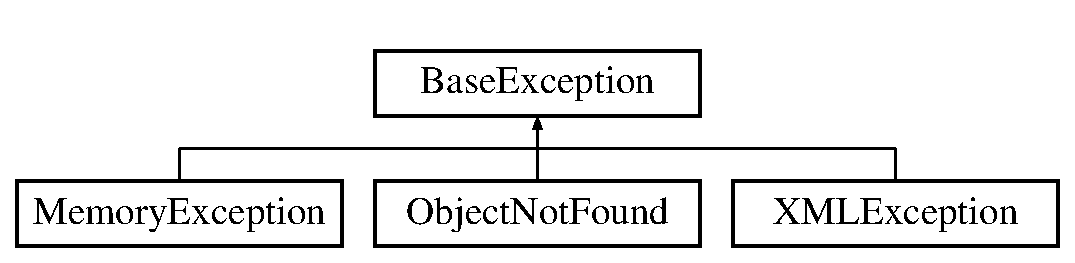
\includegraphics[height=2.000000cm]{structBaseException}
\end{center}
\end{figure}
\subsection*{Public Member Functions}
\begin{DoxyCompactItemize}
\item 
\hyperlink{structBaseException_afceeee9f97b6e2bed459692b4050f1a9}{BaseException} (const std::string \&val)
\item 
\hyperlink{structBaseException_aed58cb09c64408372719754da40022fc}{$\sim$BaseException} ()  throw ()
\item 
const char $\ast$ \hyperlink{structBaseException_a44505abd2e88ffaf5bb90e73452151b6}{what} () const   throw ()
\end{DoxyCompactItemize}
\subsection*{Public Attributes}
\begin{DoxyCompactItemize}
\item 
std::string \hyperlink{structBaseException_a0e59e8c1ac3653ba4c375e446b6a0462}{str}
\end{DoxyCompactItemize}


\subsection{Detailed Description}
Base exception. All other exceptions inherit this exception for easy filtering of exceptions

Extra functionality: the object takes a std::string parameter for customising the error message and returns this string (as a C-\/string) in the \hyperlink{structBaseException_a44505abd2e88ffaf5bb90e73452151b6}{what()} method. 

Definition at line 18 of file Exceptions.h.



\subsection{Constructor \& Destructor Documentation}
\hypertarget{structBaseException_afceeee9f97b6e2bed459692b4050f1a9}{
\index{BaseException@{BaseException}!BaseException@{BaseException}}
\index{BaseException@{BaseException}!BaseException@{BaseException}}
\subsubsection[{BaseException}]{\setlength{\rightskip}{0pt plus 5cm}BaseException::BaseException (
\begin{DoxyParamCaption}
\item[{const std::string \&}]{ val}
\end{DoxyParamCaption}
)\hspace{0.3cm}{\ttfamily  \mbox{[}inline\mbox{]}}}}
\label{structBaseException_afceeee9f97b6e2bed459692b4050f1a9}


Definition at line 21 of file Exceptions.h.

\hypertarget{structBaseException_aed58cb09c64408372719754da40022fc}{
\index{BaseException@{BaseException}!$\sim$BaseException@{$\sim$BaseException}}
\index{$\sim$BaseException@{$\sim$BaseException}!BaseException@{BaseException}}
\subsubsection[{$\sim$BaseException}]{\setlength{\rightskip}{0pt plus 5cm}BaseException::$\sim$BaseException (
\begin{DoxyParamCaption}
{}
\end{DoxyParamCaption}
)  throw ()\hspace{0.3cm}{\ttfamily  \mbox{[}inline\mbox{]}}}}
\label{structBaseException_aed58cb09c64408372719754da40022fc}


Definition at line 22 of file Exceptions.h.



\subsection{Member Function Documentation}
\hypertarget{structBaseException_a44505abd2e88ffaf5bb90e73452151b6}{
\index{BaseException@{BaseException}!what@{what}}
\index{what@{what}!BaseException@{BaseException}}
\subsubsection[{what}]{\setlength{\rightskip}{0pt plus 5cm}const char$\ast$ BaseException::what (
\begin{DoxyParamCaption}
{}
\end{DoxyParamCaption}
) const  throw ()\hspace{0.3cm}{\ttfamily  \mbox{[}inline\mbox{]}}}}
\label{structBaseException_a44505abd2e88ffaf5bb90e73452151b6}


Definition at line 23 of file Exceptions.h.



\subsection{Member Data Documentation}
\hypertarget{structBaseException_a0e59e8c1ac3653ba4c375e446b6a0462}{
\index{BaseException@{BaseException}!str@{str}}
\index{str@{str}!BaseException@{BaseException}}
\subsubsection[{str}]{\setlength{\rightskip}{0pt plus 5cm}std::string {\bf BaseException::str}}}
\label{structBaseException_a0e59e8c1ac3653ba4c375e446b6a0462}


Definition at line 20 of file Exceptions.h.



The documentation for this struct was generated from the following file:\begin{DoxyCompactItemize}
\item 
include/\hyperlink{Exceptions_8h}{Exceptions.h}\end{DoxyCompactItemize}

\hypertarget{classConfig_1_1Config}{
\section{Config::Config Class Reference}
\label{classConfig_1_1Config}\index{Config::Config@{Config::Config}}
}


XML configuration file parser.  




{\ttfamily \#include $<$XMLParserPugi.h$>$}

\subsection*{Public Member Functions}
\begin{DoxyCompactItemize}
\item 
\hyperlink{classConfig_1_1Config_a2029fc9e053c01997e11e12a37c0fa6d}{Config} ()
\item 
virtual \hyperlink{classConfig_1_1Config_af79503333d9b5121ecce39cb6dd37d0a}{$\sim$Config} ()
\item 
void \hyperlink{classConfig_1_1Config_a265403655a8e7eeb6e1f6ea98a2bc972}{LoadFromFile} (const string \&filename)
\item 
void \hyperlink{classConfig_1_1Config_a63a4269e2f438b77f336abaa2e787228}{LoadFromMemory} (const string \&chars)
\item 
vector$<$ double $>$ \& \hyperlink{classConfig_1_1Config_ab956caec2523388a0a5d94e7d7adcefe}{getCoeffs} ()
\item 
int \hyperlink{classConfig_1_1Config_ababbbc7dc47e8cc17ae55eec2f335994}{getId} ()
\item 
double \hyperlink{classConfig_1_1Config_a33ecdf7de0dfcafbc63a50c0231c074d}{getPlanetRadius} ()
\item 
double \hyperlink{classConfig_1_1Config_a2aafbc9d5be8e6f97070df517ca58552}{getStarRadius} ()
\item 
double \hyperlink{classConfig_1_1Config_a238734845144395728afea0cf4d499a9}{getPeriod} ()
\item 
double \hyperlink{classConfig_1_1Config_a94d5624d0d2f127ec00d560ccac121f8}{getSemi} ()
\item 
double \hyperlink{classConfig_1_1Config_a15d450e32246e7bb5439c0cfe68dedfd}{getInclination} ()
\item 
double \hyperlink{classConfig_1_1Config_a91cbcd53b8bbb260603f36959b419bee}{getMaxTime} ()
\item 
double \hyperlink{classConfig_1_1Config_a07c405b7013694fea51eb7d902ad4abb}{getDT} ()
\item 
double \hyperlink{classConfig_1_1Config_a93247745f2020ef250453fd9b61b4cb4}{getDR} ()
\item 
double \hyperlink{classConfig_1_1Config_add5d144f8f59e3737f0c88f4deb2669e}{getMidpoint} ()
\item 
double \hyperlink{classConfig_1_1Config_a6d86b540ec8b4264fa3d3e00065ce2a5}{getNoise} ()
\end{DoxyCompactItemize}
\subsection*{Protected Member Functions}
\begin{DoxyCompactItemize}
\item 
void \hyperlink{classConfig_1_1Config_ab2f28785892ab6bea1af4df4d4caf93a}{m\_\-getPlanetRadius} ()
\item 
void \hyperlink{classConfig_1_1Config_a54e1763c19f3d2418005a2419cb9eb27}{m\_\-getStarRadius} ()
\item 
void \hyperlink{classConfig_1_1Config_a885f61f26d416fc460fcb01ae79e5a05}{m\_\-getLDCoeffs} ()
\item 
void \hyperlink{classConfig_1_1Config_a2341de58cf443afd26c4b258d0a287ea}{m\_\-getPeriod} ()
\item 
void \hyperlink{classConfig_1_1Config_a19d12b578cebc897ad0c5aaafc391f6a}{m\_\-getSemi} ()
\item 
void \hyperlink{classConfig_1_1Config_a4ce8f61abcabce4ccad266d58cc27bdd}{m\_\-getInclination} ()
\item 
void \hyperlink{classConfig_1_1Config_a178d0dbcf71e20379a9269dc6e403539}{m\_\-getMaxTime} ()
\item 
void \hyperlink{classConfig_1_1Config_a902f1fcfd33f840b45d9973402e928ce}{m\_\-getDT} ()
\item 
void \hyperlink{classConfig_1_1Config_a7b847ddb671a80c3e9234f070e8d7f06}{m\_\-getDR} ()
\item 
void \hyperlink{classConfig_1_1Config_adbb674970bddcda634ec49fd168b43e7}{m\_\-getMidpoint} ()
\item 
void \hyperlink{classConfig_1_1Config_a191605695b16e5a91d8f989b0c6e2d43}{m\_\-getNoise} ()
\item 
void \hyperlink{classConfig_1_1Config_aeb68940be8481ce24555f294b5e72570}{m\_\-getAll} ()
\begin{DoxyCompactList}\small\item\em Global data retrieval function. \item\end{DoxyCompactList}\item 
void \hyperlink{classConfig_1_1Config_ad83da68d740dac994311fedd2d85c412}{init} ()
\end{DoxyCompactItemize}
\subsection*{Private Attributes}
\begin{DoxyCompactItemize}
\item 
vector$<$ double $>$ \hyperlink{classConfig_1_1Config_a9c679f504309dbeb9f0888f40df2c36b}{coeffs}
\item 
int \hyperlink{classConfig_1_1Config_ae54078b2b14014b3b1bba13fc9aa2fa9}{id}
\item 
double \hyperlink{classConfig_1_1Config_aa7f8b446e7c7db6ab117de7bb12e8193}{planetRadius}
\item 
double \hyperlink{classConfig_1_1Config_a2420c3fc48cec4f14644afb532ffcf39}{starRadius}
\item 
double \hyperlink{classConfig_1_1Config_afc6907d04c9ccbf1479845699943c3bc}{period}
\item 
double \hyperlink{classConfig_1_1Config_ac226b3dfdaf293240a6bfceb3b195d88}{semi}
\item 
double \hyperlink{classConfig_1_1Config_adb71ce5d055b439fa0c3641c6400327e}{inclination}
\item 
double \hyperlink{classConfig_1_1Config_a3dcb214d120167f7bb6902892942d831}{maxtime}
\item 
double \hyperlink{classConfig_1_1Config_a37c6fb687d364836452dc746be9bc0cb}{dt}
\item 
double \hyperlink{classConfig_1_1Config_ab116322f18f71b98be1ab00413edc400}{dr}
\item 
double \hyperlink{classConfig_1_1Config_ada14b015b08c65e217d223fead656748}{midpoint}
\item 
double \hyperlink{classConfig_1_1Config_a0e9e59c906c710bb12efe8a620502109}{noise}
\item 
pugi::xml\_\-document \hyperlink{classConfig_1_1Config_a61dfb08aaa9e051084d7c94cbe2d23b5}{doc}
\begin{DoxyCompactList}\small\item\em Document node. \item\end{DoxyCompactList}\item 
pugi::xml\_\-parse\_\-result \hyperlink{classConfig_1_1Config_adc7aa2f037d2b6c7f377b2ac2ec0e1b1}{result}
\begin{DoxyCompactList}\small\item\em Result of the xml parsing. \item\end{DoxyCompactList}\item 
pugi::xml\_\-node \hyperlink{classConfig_1_1Config_a86646003839a5b91e5c9281bb0c65e4a}{PlanetNode}
\begin{DoxyCompactList}\small\item\em Planetary parameter node. \item\end{DoxyCompactList}\item 
pugi::xml\_\-node \hyperlink{classConfig_1_1Config_ae031c18b0ec9ff285a88341b2a9da6d3}{StarNode}
\begin{DoxyCompactList}\small\item\em Stellar parameter node. \item\end{DoxyCompactList}\item 
pugi::xml\_\-node \hyperlink{classConfig_1_1Config_a5b48e9e8de00ec0f85d7ac2bae12212d}{OrbitNode}
\begin{DoxyCompactList}\small\item\em Orbital parameter node. \item\end{DoxyCompactList}\item 
pugi::xml\_\-node \hyperlink{classConfig_1_1Config_a116dd11fe52f850709971ba73b8f7560}{SimulationNode}
\begin{DoxyCompactList}\small\item\em Simulation information node. \item\end{DoxyCompactList}\end{DoxyCompactItemize}


\subsection{Detailed Description}
XML configuration file parser. This file reads in the simulation configuration parameters in from the specified xml file and stores all the required variables in its own memory space for later access. 

Definition at line 29 of file XMLParserPugi.h.



\subsection{Constructor \& Destructor Documentation}
\hypertarget{classConfig_1_1Config_a2029fc9e053c01997e11e12a37c0fa6d}{
\index{Config::Config@{Config::Config}!Config@{Config}}
\index{Config@{Config}!Config::Config@{Config::Config}}
\subsubsection[{Config}]{\setlength{\rightskip}{0pt plus 5cm}Config::Config::Config (
\begin{DoxyParamCaption}
{}
\end{DoxyParamCaption}
)}}
\label{classConfig_1_1Config_a2029fc9e053c01997e11e12a37c0fa6d}
\hypertarget{classConfig_1_1Config_af79503333d9b5121ecce39cb6dd37d0a}{
\index{Config::Config@{Config::Config}!$\sim$Config@{$\sim$Config}}
\index{$\sim$Config@{$\sim$Config}!Config::Config@{Config::Config}}
\subsubsection[{$\sim$Config}]{\setlength{\rightskip}{0pt plus 5cm}virtual Config::Config::$\sim$Config (
\begin{DoxyParamCaption}
{}
\end{DoxyParamCaption}
)\hspace{0.3cm}{\ttfamily  \mbox{[}virtual\mbox{]}}}}
\label{classConfig_1_1Config_af79503333d9b5121ecce39cb6dd37d0a}


\subsection{Member Function Documentation}
\hypertarget{classConfig_1_1Config_ab956caec2523388a0a5d94e7d7adcefe}{
\index{Config::Config@{Config::Config}!getCoeffs@{getCoeffs}}
\index{getCoeffs@{getCoeffs}!Config::Config@{Config::Config}}
\subsubsection[{getCoeffs}]{\setlength{\rightskip}{0pt plus 5cm}vector$<$double$>$\& Config::Config::getCoeffs (
\begin{DoxyParamCaption}
{}
\end{DoxyParamCaption}
)\hspace{0.3cm}{\ttfamily  \mbox{[}inline\mbox{]}}}}
\label{classConfig_1_1Config_ab956caec2523388a0a5d94e7d7adcefe}


Definition at line 90 of file XMLParserPugi.h.

\hypertarget{classConfig_1_1Config_a93247745f2020ef250453fd9b61b4cb4}{
\index{Config::Config@{Config::Config}!getDR@{getDR}}
\index{getDR@{getDR}!Config::Config@{Config::Config}}
\subsubsection[{getDR}]{\setlength{\rightskip}{0pt plus 5cm}double Config::Config::getDR (
\begin{DoxyParamCaption}
{}
\end{DoxyParamCaption}
)\hspace{0.3cm}{\ttfamily  \mbox{[}inline\mbox{]}}}}
\label{classConfig_1_1Config_a93247745f2020ef250453fd9b61b4cb4}


Definition at line 99 of file XMLParserPugi.h.

\hypertarget{classConfig_1_1Config_a07c405b7013694fea51eb7d902ad4abb}{
\index{Config::Config@{Config::Config}!getDT@{getDT}}
\index{getDT@{getDT}!Config::Config@{Config::Config}}
\subsubsection[{getDT}]{\setlength{\rightskip}{0pt plus 5cm}double Config::Config::getDT (
\begin{DoxyParamCaption}
{}
\end{DoxyParamCaption}
)\hspace{0.3cm}{\ttfamily  \mbox{[}inline\mbox{]}}}}
\label{classConfig_1_1Config_a07c405b7013694fea51eb7d902ad4abb}


Definition at line 98 of file XMLParserPugi.h.

\hypertarget{classConfig_1_1Config_ababbbc7dc47e8cc17ae55eec2f335994}{
\index{Config::Config@{Config::Config}!getId@{getId}}
\index{getId@{getId}!Config::Config@{Config::Config}}
\subsubsection[{getId}]{\setlength{\rightskip}{0pt plus 5cm}int Config::Config::getId (
\begin{DoxyParamCaption}
{}
\end{DoxyParamCaption}
)\hspace{0.3cm}{\ttfamily  \mbox{[}inline\mbox{]}}}}
\label{classConfig_1_1Config_ababbbc7dc47e8cc17ae55eec2f335994}


Definition at line 91 of file XMLParserPugi.h.

\hypertarget{classConfig_1_1Config_a15d450e32246e7bb5439c0cfe68dedfd}{
\index{Config::Config@{Config::Config}!getInclination@{getInclination}}
\index{getInclination@{getInclination}!Config::Config@{Config::Config}}
\subsubsection[{getInclination}]{\setlength{\rightskip}{0pt plus 5cm}double Config::Config::getInclination (
\begin{DoxyParamCaption}
{}
\end{DoxyParamCaption}
)\hspace{0.3cm}{\ttfamily  \mbox{[}inline\mbox{]}}}}
\label{classConfig_1_1Config_a15d450e32246e7bb5439c0cfe68dedfd}


Definition at line 96 of file XMLParserPugi.h.

\hypertarget{classConfig_1_1Config_a91cbcd53b8bbb260603f36959b419bee}{
\index{Config::Config@{Config::Config}!getMaxTime@{getMaxTime}}
\index{getMaxTime@{getMaxTime}!Config::Config@{Config::Config}}
\subsubsection[{getMaxTime}]{\setlength{\rightskip}{0pt plus 5cm}double Config::Config::getMaxTime (
\begin{DoxyParamCaption}
{}
\end{DoxyParamCaption}
)\hspace{0.3cm}{\ttfamily  \mbox{[}inline\mbox{]}}}}
\label{classConfig_1_1Config_a91cbcd53b8bbb260603f36959b419bee}


Definition at line 97 of file XMLParserPugi.h.

\hypertarget{classConfig_1_1Config_add5d144f8f59e3737f0c88f4deb2669e}{
\index{Config::Config@{Config::Config}!getMidpoint@{getMidpoint}}
\index{getMidpoint@{getMidpoint}!Config::Config@{Config::Config}}
\subsubsection[{getMidpoint}]{\setlength{\rightskip}{0pt plus 5cm}double Config::Config::getMidpoint (
\begin{DoxyParamCaption}
{}
\end{DoxyParamCaption}
)\hspace{0.3cm}{\ttfamily  \mbox{[}inline\mbox{]}}}}
\label{classConfig_1_1Config_add5d144f8f59e3737f0c88f4deb2669e}


Definition at line 100 of file XMLParserPugi.h.

\hypertarget{classConfig_1_1Config_a6d86b540ec8b4264fa3d3e00065ce2a5}{
\index{Config::Config@{Config::Config}!getNoise@{getNoise}}
\index{getNoise@{getNoise}!Config::Config@{Config::Config}}
\subsubsection[{getNoise}]{\setlength{\rightskip}{0pt plus 5cm}double Config::Config::getNoise (
\begin{DoxyParamCaption}
{}
\end{DoxyParamCaption}
)\hspace{0.3cm}{\ttfamily  \mbox{[}inline\mbox{]}}}}
\label{classConfig_1_1Config_a6d86b540ec8b4264fa3d3e00065ce2a5}


Definition at line 101 of file XMLParserPugi.h.

\hypertarget{classConfig_1_1Config_a238734845144395728afea0cf4d499a9}{
\index{Config::Config@{Config::Config}!getPeriod@{getPeriod}}
\index{getPeriod@{getPeriod}!Config::Config@{Config::Config}}
\subsubsection[{getPeriod}]{\setlength{\rightskip}{0pt plus 5cm}double Config::Config::getPeriod (
\begin{DoxyParamCaption}
{}
\end{DoxyParamCaption}
)\hspace{0.3cm}{\ttfamily  \mbox{[}inline\mbox{]}}}}
\label{classConfig_1_1Config_a238734845144395728afea0cf4d499a9}


Definition at line 94 of file XMLParserPugi.h.

\hypertarget{classConfig_1_1Config_a33ecdf7de0dfcafbc63a50c0231c074d}{
\index{Config::Config@{Config::Config}!getPlanetRadius@{getPlanetRadius}}
\index{getPlanetRadius@{getPlanetRadius}!Config::Config@{Config::Config}}
\subsubsection[{getPlanetRadius}]{\setlength{\rightskip}{0pt plus 5cm}double Config::Config::getPlanetRadius (
\begin{DoxyParamCaption}
{}
\end{DoxyParamCaption}
)\hspace{0.3cm}{\ttfamily  \mbox{[}inline\mbox{]}}}}
\label{classConfig_1_1Config_a33ecdf7de0dfcafbc63a50c0231c074d}


Definition at line 92 of file XMLParserPugi.h.

\hypertarget{classConfig_1_1Config_a94d5624d0d2f127ec00d560ccac121f8}{
\index{Config::Config@{Config::Config}!getSemi@{getSemi}}
\index{getSemi@{getSemi}!Config::Config@{Config::Config}}
\subsubsection[{getSemi}]{\setlength{\rightskip}{0pt plus 5cm}double Config::Config::getSemi (
\begin{DoxyParamCaption}
{}
\end{DoxyParamCaption}
)\hspace{0.3cm}{\ttfamily  \mbox{[}inline\mbox{]}}}}
\label{classConfig_1_1Config_a94d5624d0d2f127ec00d560ccac121f8}


Definition at line 95 of file XMLParserPugi.h.

\hypertarget{classConfig_1_1Config_a2aafbc9d5be8e6f97070df517ca58552}{
\index{Config::Config@{Config::Config}!getStarRadius@{getStarRadius}}
\index{getStarRadius@{getStarRadius}!Config::Config@{Config::Config}}
\subsubsection[{getStarRadius}]{\setlength{\rightskip}{0pt plus 5cm}double Config::Config::getStarRadius (
\begin{DoxyParamCaption}
{}
\end{DoxyParamCaption}
)\hspace{0.3cm}{\ttfamily  \mbox{[}inline\mbox{]}}}}
\label{classConfig_1_1Config_a2aafbc9d5be8e6f97070df517ca58552}


Definition at line 93 of file XMLParserPugi.h.

\hypertarget{classConfig_1_1Config_ad83da68d740dac994311fedd2d85c412}{
\index{Config::Config@{Config::Config}!init@{init}}
\index{init@{init}!Config::Config@{Config::Config}}
\subsubsection[{init}]{\setlength{\rightskip}{0pt plus 5cm}void Config::Config::init (
\begin{DoxyParamCaption}
{}
\end{DoxyParamCaption}
)\hspace{0.3cm}{\ttfamily  \mbox{[}protected\mbox{]}}}}
\label{classConfig_1_1Config_ad83da68d740dac994311fedd2d85c412}
\hypertarget{classConfig_1_1Config_a265403655a8e7eeb6e1f6ea98a2bc972}{
\index{Config::Config@{Config::Config}!LoadFromFile@{LoadFromFile}}
\index{LoadFromFile@{LoadFromFile}!Config::Config@{Config::Config}}
\subsubsection[{LoadFromFile}]{\setlength{\rightskip}{0pt plus 5cm}void Config::Config::LoadFromFile (
\begin{DoxyParamCaption}
\item[{const string \&}]{ filename}
\end{DoxyParamCaption}
)}}
\label{classConfig_1_1Config_a265403655a8e7eeb6e1f6ea98a2bc972}
\hypertarget{classConfig_1_1Config_a63a4269e2f438b77f336abaa2e787228}{
\index{Config::Config@{Config::Config}!LoadFromMemory@{LoadFromMemory}}
\index{LoadFromMemory@{LoadFromMemory}!Config::Config@{Config::Config}}
\subsubsection[{LoadFromMemory}]{\setlength{\rightskip}{0pt plus 5cm}void Config::Config::LoadFromMemory (
\begin{DoxyParamCaption}
\item[{const string \&}]{ chars}
\end{DoxyParamCaption}
)}}
\label{classConfig_1_1Config_a63a4269e2f438b77f336abaa2e787228}
\hypertarget{classConfig_1_1Config_aeb68940be8481ce24555f294b5e72570}{
\index{Config::Config@{Config::Config}!m\_\-getAll@{m\_\-getAll}}
\index{m\_\-getAll@{m\_\-getAll}!Config::Config@{Config::Config}}
\subsubsection[{m\_\-getAll}]{\setlength{\rightskip}{0pt plus 5cm}void Config::Config::m\_\-getAll (
\begin{DoxyParamCaption}
{}
\end{DoxyParamCaption}
)\hspace{0.3cm}{\ttfamily  \mbox{[}protected\mbox{]}}}}
\label{classConfig_1_1Config_aeb68940be8481ce24555f294b5e72570}


Global data retrieval function. 

\hypertarget{classConfig_1_1Config_a7b847ddb671a80c3e9234f070e8d7f06}{
\index{Config::Config@{Config::Config}!m\_\-getDR@{m\_\-getDR}}
\index{m\_\-getDR@{m\_\-getDR}!Config::Config@{Config::Config}}
\subsubsection[{m\_\-getDR}]{\setlength{\rightskip}{0pt plus 5cm}void Config::Config::m\_\-getDR (
\begin{DoxyParamCaption}
{}
\end{DoxyParamCaption}
)\hspace{0.3cm}{\ttfamily  \mbox{[}protected\mbox{]}}}}
\label{classConfig_1_1Config_a7b847ddb671a80c3e9234f070e8d7f06}
\hypertarget{classConfig_1_1Config_a902f1fcfd33f840b45d9973402e928ce}{
\index{Config::Config@{Config::Config}!m\_\-getDT@{m\_\-getDT}}
\index{m\_\-getDT@{m\_\-getDT}!Config::Config@{Config::Config}}
\subsubsection[{m\_\-getDT}]{\setlength{\rightskip}{0pt plus 5cm}void Config::Config::m\_\-getDT (
\begin{DoxyParamCaption}
{}
\end{DoxyParamCaption}
)\hspace{0.3cm}{\ttfamily  \mbox{[}protected\mbox{]}}}}
\label{classConfig_1_1Config_a902f1fcfd33f840b45d9973402e928ce}
\hypertarget{classConfig_1_1Config_a4ce8f61abcabce4ccad266d58cc27bdd}{
\index{Config::Config@{Config::Config}!m\_\-getInclination@{m\_\-getInclination}}
\index{m\_\-getInclination@{m\_\-getInclination}!Config::Config@{Config::Config}}
\subsubsection[{m\_\-getInclination}]{\setlength{\rightskip}{0pt plus 5cm}void Config::Config::m\_\-getInclination (
\begin{DoxyParamCaption}
{}
\end{DoxyParamCaption}
)\hspace{0.3cm}{\ttfamily  \mbox{[}protected\mbox{]}}}}
\label{classConfig_1_1Config_a4ce8f61abcabce4ccad266d58cc27bdd}
\hypertarget{classConfig_1_1Config_a885f61f26d416fc460fcb01ae79e5a05}{
\index{Config::Config@{Config::Config}!m\_\-getLDCoeffs@{m\_\-getLDCoeffs}}
\index{m\_\-getLDCoeffs@{m\_\-getLDCoeffs}!Config::Config@{Config::Config}}
\subsubsection[{m\_\-getLDCoeffs}]{\setlength{\rightskip}{0pt plus 5cm}void Config::Config::m\_\-getLDCoeffs (
\begin{DoxyParamCaption}
{}
\end{DoxyParamCaption}
)\hspace{0.3cm}{\ttfamily  \mbox{[}protected\mbox{]}}}}
\label{classConfig_1_1Config_a885f61f26d416fc460fcb01ae79e5a05}
\hypertarget{classConfig_1_1Config_a178d0dbcf71e20379a9269dc6e403539}{
\index{Config::Config@{Config::Config}!m\_\-getMaxTime@{m\_\-getMaxTime}}
\index{m\_\-getMaxTime@{m\_\-getMaxTime}!Config::Config@{Config::Config}}
\subsubsection[{m\_\-getMaxTime}]{\setlength{\rightskip}{0pt plus 5cm}void Config::Config::m\_\-getMaxTime (
\begin{DoxyParamCaption}
{}
\end{DoxyParamCaption}
)\hspace{0.3cm}{\ttfamily  \mbox{[}protected\mbox{]}}}}
\label{classConfig_1_1Config_a178d0dbcf71e20379a9269dc6e403539}
\hypertarget{classConfig_1_1Config_adbb674970bddcda634ec49fd168b43e7}{
\index{Config::Config@{Config::Config}!m\_\-getMidpoint@{m\_\-getMidpoint}}
\index{m\_\-getMidpoint@{m\_\-getMidpoint}!Config::Config@{Config::Config}}
\subsubsection[{m\_\-getMidpoint}]{\setlength{\rightskip}{0pt plus 5cm}void Config::Config::m\_\-getMidpoint (
\begin{DoxyParamCaption}
{}
\end{DoxyParamCaption}
)\hspace{0.3cm}{\ttfamily  \mbox{[}protected\mbox{]}}}}
\label{classConfig_1_1Config_adbb674970bddcda634ec49fd168b43e7}
\hypertarget{classConfig_1_1Config_a191605695b16e5a91d8f989b0c6e2d43}{
\index{Config::Config@{Config::Config}!m\_\-getNoise@{m\_\-getNoise}}
\index{m\_\-getNoise@{m\_\-getNoise}!Config::Config@{Config::Config}}
\subsubsection[{m\_\-getNoise}]{\setlength{\rightskip}{0pt plus 5cm}void Config::Config::m\_\-getNoise (
\begin{DoxyParamCaption}
{}
\end{DoxyParamCaption}
)\hspace{0.3cm}{\ttfamily  \mbox{[}protected\mbox{]}}}}
\label{classConfig_1_1Config_a191605695b16e5a91d8f989b0c6e2d43}
\hypertarget{classConfig_1_1Config_a2341de58cf443afd26c4b258d0a287ea}{
\index{Config::Config@{Config::Config}!m\_\-getPeriod@{m\_\-getPeriod}}
\index{m\_\-getPeriod@{m\_\-getPeriod}!Config::Config@{Config::Config}}
\subsubsection[{m\_\-getPeriod}]{\setlength{\rightskip}{0pt plus 5cm}void Config::Config::m\_\-getPeriod (
\begin{DoxyParamCaption}
{}
\end{DoxyParamCaption}
)\hspace{0.3cm}{\ttfamily  \mbox{[}protected\mbox{]}}}}
\label{classConfig_1_1Config_a2341de58cf443afd26c4b258d0a287ea}
\hypertarget{classConfig_1_1Config_ab2f28785892ab6bea1af4df4d4caf93a}{
\index{Config::Config@{Config::Config}!m\_\-getPlanetRadius@{m\_\-getPlanetRadius}}
\index{m\_\-getPlanetRadius@{m\_\-getPlanetRadius}!Config::Config@{Config::Config}}
\subsubsection[{m\_\-getPlanetRadius}]{\setlength{\rightskip}{0pt plus 5cm}void Config::Config::m\_\-getPlanetRadius (
\begin{DoxyParamCaption}
{}
\end{DoxyParamCaption}
)\hspace{0.3cm}{\ttfamily  \mbox{[}protected\mbox{]}}}}
\label{classConfig_1_1Config_ab2f28785892ab6bea1af4df4d4caf93a}
\hypertarget{classConfig_1_1Config_a19d12b578cebc897ad0c5aaafc391f6a}{
\index{Config::Config@{Config::Config}!m\_\-getSemi@{m\_\-getSemi}}
\index{m\_\-getSemi@{m\_\-getSemi}!Config::Config@{Config::Config}}
\subsubsection[{m\_\-getSemi}]{\setlength{\rightskip}{0pt plus 5cm}void Config::Config::m\_\-getSemi (
\begin{DoxyParamCaption}
{}
\end{DoxyParamCaption}
)\hspace{0.3cm}{\ttfamily  \mbox{[}protected\mbox{]}}}}
\label{classConfig_1_1Config_a19d12b578cebc897ad0c5aaafc391f6a}
\hypertarget{classConfig_1_1Config_a54e1763c19f3d2418005a2419cb9eb27}{
\index{Config::Config@{Config::Config}!m\_\-getStarRadius@{m\_\-getStarRadius}}
\index{m\_\-getStarRadius@{m\_\-getStarRadius}!Config::Config@{Config::Config}}
\subsubsection[{m\_\-getStarRadius}]{\setlength{\rightskip}{0pt plus 5cm}void Config::Config::m\_\-getStarRadius (
\begin{DoxyParamCaption}
{}
\end{DoxyParamCaption}
)\hspace{0.3cm}{\ttfamily  \mbox{[}protected\mbox{]}}}}
\label{classConfig_1_1Config_a54e1763c19f3d2418005a2419cb9eb27}


\subsection{Member Data Documentation}
\hypertarget{classConfig_1_1Config_a9c679f504309dbeb9f0888f40df2c36b}{
\index{Config::Config@{Config::Config}!coeffs@{coeffs}}
\index{coeffs@{coeffs}!Config::Config@{Config::Config}}
\subsubsection[{coeffs}]{\setlength{\rightskip}{0pt plus 5cm}vector$<$double$>$ {\bf Config::Config::coeffs}\hspace{0.3cm}{\ttfamily  \mbox{[}private\mbox{]}}}}
\label{classConfig_1_1Config_a9c679f504309dbeb9f0888f40df2c36b}


Definition at line 31 of file XMLParserPugi.h.

\hypertarget{classConfig_1_1Config_a61dfb08aaa9e051084d7c94cbe2d23b5}{
\index{Config::Config@{Config::Config}!doc@{doc}}
\index{doc@{doc}!Config::Config@{Config::Config}}
\subsubsection[{doc}]{\setlength{\rightskip}{0pt plus 5cm}pugi::xml\_\-document {\bf Config::Config::doc}\hspace{0.3cm}{\ttfamily  \mbox{[}private\mbox{]}}}}
\label{classConfig_1_1Config_a61dfb08aaa9e051084d7c94cbe2d23b5}


Document node. 



Definition at line 46 of file XMLParserPugi.h.

\hypertarget{classConfig_1_1Config_ab116322f18f71b98be1ab00413edc400}{
\index{Config::Config@{Config::Config}!dr@{dr}}
\index{dr@{dr}!Config::Config@{Config::Config}}
\subsubsection[{dr}]{\setlength{\rightskip}{0pt plus 5cm}double {\bf Config::Config::dr}\hspace{0.3cm}{\ttfamily  \mbox{[}private\mbox{]}}}}
\label{classConfig_1_1Config_ab116322f18f71b98be1ab00413edc400}


Definition at line 40 of file XMLParserPugi.h.

\hypertarget{classConfig_1_1Config_a37c6fb687d364836452dc746be9bc0cb}{
\index{Config::Config@{Config::Config}!dt@{dt}}
\index{dt@{dt}!Config::Config@{Config::Config}}
\subsubsection[{dt}]{\setlength{\rightskip}{0pt plus 5cm}double {\bf Config::Config::dt}\hspace{0.3cm}{\ttfamily  \mbox{[}private\mbox{]}}}}
\label{classConfig_1_1Config_a37c6fb687d364836452dc746be9bc0cb}


Definition at line 39 of file XMLParserPugi.h.

\hypertarget{classConfig_1_1Config_ae54078b2b14014b3b1bba13fc9aa2fa9}{
\index{Config::Config@{Config::Config}!id@{id}}
\index{id@{id}!Config::Config@{Config::Config}}
\subsubsection[{id}]{\setlength{\rightskip}{0pt plus 5cm}int {\bf Config::Config::id}\hspace{0.3cm}{\ttfamily  \mbox{[}private\mbox{]}}}}
\label{classConfig_1_1Config_ae54078b2b14014b3b1bba13fc9aa2fa9}


Definition at line 32 of file XMLParserPugi.h.

\hypertarget{classConfig_1_1Config_adb71ce5d055b439fa0c3641c6400327e}{
\index{Config::Config@{Config::Config}!inclination@{inclination}}
\index{inclination@{inclination}!Config::Config@{Config::Config}}
\subsubsection[{inclination}]{\setlength{\rightskip}{0pt plus 5cm}double {\bf Config::Config::inclination}\hspace{0.3cm}{\ttfamily  \mbox{[}private\mbox{]}}}}
\label{classConfig_1_1Config_adb71ce5d055b439fa0c3641c6400327e}


Definition at line 37 of file XMLParserPugi.h.

\hypertarget{classConfig_1_1Config_a3dcb214d120167f7bb6902892942d831}{
\index{Config::Config@{Config::Config}!maxtime@{maxtime}}
\index{maxtime@{maxtime}!Config::Config@{Config::Config}}
\subsubsection[{maxtime}]{\setlength{\rightskip}{0pt plus 5cm}double {\bf Config::Config::maxtime}\hspace{0.3cm}{\ttfamily  \mbox{[}private\mbox{]}}}}
\label{classConfig_1_1Config_a3dcb214d120167f7bb6902892942d831}


Definition at line 38 of file XMLParserPugi.h.

\hypertarget{classConfig_1_1Config_ada14b015b08c65e217d223fead656748}{
\index{Config::Config@{Config::Config}!midpoint@{midpoint}}
\index{midpoint@{midpoint}!Config::Config@{Config::Config}}
\subsubsection[{midpoint}]{\setlength{\rightskip}{0pt plus 5cm}double {\bf Config::Config::midpoint}\hspace{0.3cm}{\ttfamily  \mbox{[}private\mbox{]}}}}
\label{classConfig_1_1Config_ada14b015b08c65e217d223fead656748}


Definition at line 41 of file XMLParserPugi.h.

\hypertarget{classConfig_1_1Config_a0e9e59c906c710bb12efe8a620502109}{
\index{Config::Config@{Config::Config}!noise@{noise}}
\index{noise@{noise}!Config::Config@{Config::Config}}
\subsubsection[{noise}]{\setlength{\rightskip}{0pt plus 5cm}double {\bf Config::Config::noise}\hspace{0.3cm}{\ttfamily  \mbox{[}private\mbox{]}}}}
\label{classConfig_1_1Config_a0e9e59c906c710bb12efe8a620502109}


Definition at line 42 of file XMLParserPugi.h.

\hypertarget{classConfig_1_1Config_a5b48e9e8de00ec0f85d7ac2bae12212d}{
\index{Config::Config@{Config::Config}!OrbitNode@{OrbitNode}}
\index{OrbitNode@{OrbitNode}!Config::Config@{Config::Config}}
\subsubsection[{OrbitNode}]{\setlength{\rightskip}{0pt plus 5cm}pugi::xml\_\-node {\bf Config::Config::OrbitNode}\hspace{0.3cm}{\ttfamily  \mbox{[}private\mbox{]}}}}
\label{classConfig_1_1Config_a5b48e9e8de00ec0f85d7ac2bae12212d}


Orbital parameter node. 



Definition at line 58 of file XMLParserPugi.h.

\hypertarget{classConfig_1_1Config_afc6907d04c9ccbf1479845699943c3bc}{
\index{Config::Config@{Config::Config}!period@{period}}
\index{period@{period}!Config::Config@{Config::Config}}
\subsubsection[{period}]{\setlength{\rightskip}{0pt plus 5cm}double {\bf Config::Config::period}\hspace{0.3cm}{\ttfamily  \mbox{[}private\mbox{]}}}}
\label{classConfig_1_1Config_afc6907d04c9ccbf1479845699943c3bc}


Definition at line 35 of file XMLParserPugi.h.

\hypertarget{classConfig_1_1Config_a86646003839a5b91e5c9281bb0c65e4a}{
\index{Config::Config@{Config::Config}!PlanetNode@{PlanetNode}}
\index{PlanetNode@{PlanetNode}!Config::Config@{Config::Config}}
\subsubsection[{PlanetNode}]{\setlength{\rightskip}{0pt plus 5cm}pugi::xml\_\-node {\bf Config::Config::PlanetNode}\hspace{0.3cm}{\ttfamily  \mbox{[}private\mbox{]}}}}
\label{classConfig_1_1Config_a86646003839a5b91e5c9281bb0c65e4a}


Planetary parameter node. 



Definition at line 52 of file XMLParserPugi.h.

\hypertarget{classConfig_1_1Config_aa7f8b446e7c7db6ab117de7bb12e8193}{
\index{Config::Config@{Config::Config}!planetRadius@{planetRadius}}
\index{planetRadius@{planetRadius}!Config::Config@{Config::Config}}
\subsubsection[{planetRadius}]{\setlength{\rightskip}{0pt plus 5cm}double {\bf Config::Config::planetRadius}\hspace{0.3cm}{\ttfamily  \mbox{[}private\mbox{]}}}}
\label{classConfig_1_1Config_aa7f8b446e7c7db6ab117de7bb12e8193}


Definition at line 33 of file XMLParserPugi.h.

\hypertarget{classConfig_1_1Config_adc7aa2f037d2b6c7f377b2ac2ec0e1b1}{
\index{Config::Config@{Config::Config}!result@{result}}
\index{result@{result}!Config::Config@{Config::Config}}
\subsubsection[{result}]{\setlength{\rightskip}{0pt plus 5cm}pugi::xml\_\-parse\_\-result {\bf Config::Config::result}\hspace{0.3cm}{\ttfamily  \mbox{[}private\mbox{]}}}}
\label{classConfig_1_1Config_adc7aa2f037d2b6c7f377b2ac2ec0e1b1}


Result of the xml parsing. 



Definition at line 49 of file XMLParserPugi.h.

\hypertarget{classConfig_1_1Config_ac226b3dfdaf293240a6bfceb3b195d88}{
\index{Config::Config@{Config::Config}!semi@{semi}}
\index{semi@{semi}!Config::Config@{Config::Config}}
\subsubsection[{semi}]{\setlength{\rightskip}{0pt plus 5cm}double {\bf Config::Config::semi}\hspace{0.3cm}{\ttfamily  \mbox{[}private\mbox{]}}}}
\label{classConfig_1_1Config_ac226b3dfdaf293240a6bfceb3b195d88}


Definition at line 36 of file XMLParserPugi.h.

\hypertarget{classConfig_1_1Config_a116dd11fe52f850709971ba73b8f7560}{
\index{Config::Config@{Config::Config}!SimulationNode@{SimulationNode}}
\index{SimulationNode@{SimulationNode}!Config::Config@{Config::Config}}
\subsubsection[{SimulationNode}]{\setlength{\rightskip}{0pt plus 5cm}pugi::xml\_\-node {\bf Config::Config::SimulationNode}\hspace{0.3cm}{\ttfamily  \mbox{[}private\mbox{]}}}}
\label{classConfig_1_1Config_a116dd11fe52f850709971ba73b8f7560}


Simulation information node. 



Definition at line 61 of file XMLParserPugi.h.

\hypertarget{classConfig_1_1Config_ae031c18b0ec9ff285a88341b2a9da6d3}{
\index{Config::Config@{Config::Config}!StarNode@{StarNode}}
\index{StarNode@{StarNode}!Config::Config@{Config::Config}}
\subsubsection[{StarNode}]{\setlength{\rightskip}{0pt plus 5cm}pugi::xml\_\-node {\bf Config::Config::StarNode}\hspace{0.3cm}{\ttfamily  \mbox{[}private\mbox{]}}}}
\label{classConfig_1_1Config_ae031c18b0ec9ff285a88341b2a9da6d3}


Stellar parameter node. 



Definition at line 55 of file XMLParserPugi.h.

\hypertarget{classConfig_1_1Config_a2420c3fc48cec4f14644afb532ffcf39}{
\index{Config::Config@{Config::Config}!starRadius@{starRadius}}
\index{starRadius@{starRadius}!Config::Config@{Config::Config}}
\subsubsection[{starRadius}]{\setlength{\rightskip}{0pt plus 5cm}double {\bf Config::Config::starRadius}\hspace{0.3cm}{\ttfamily  \mbox{[}private\mbox{]}}}}
\label{classConfig_1_1Config_a2420c3fc48cec4f14644afb532ffcf39}


Definition at line 34 of file XMLParserPugi.h.



The documentation for this class was generated from the following file:\begin{DoxyCompactItemize}
\item 
include/\hyperlink{XMLParserPugi_8h}{XMLParserPugi.h}\end{DoxyCompactItemize}

\hypertarget{classLightcurve}{
\section{Lightcurve Class Reference}
\label{classLightcurve}\index{Lightcurve@{Lightcurve}}
}


\hyperlink{classLightcurve}{Lightcurve} class which stores information about a single object.  




{\ttfamily \#include $<$Lightcurve.h$>$}

\subsection*{Public Member Functions}
\begin{DoxyCompactItemize}
\item 
\hyperlink{classLightcurve_a1145dcf51e49e3ce069a0aad4ad11e92}{Lightcurve} (size\_\-t n)
\begin{DoxyCompactList}\small\item\em Constructor. \item\end{DoxyCompactList}\item 
void \hyperlink{classLightcurve_a5318d441e2d04d71ef10b7509f823e92}{clear} ()
\begin{DoxyCompactList}\small\item\em Manually clears the timeseries vectors. \item\end{DoxyCompactList}\item 
size\_\-t \hyperlink{classLightcurve_aa5cc8769e52679a9cc17e8c2782acbf0}{size} () const 
\begin{DoxyCompactList}\small\item\em Returns the number of data points in the lightcurve. \item\end{DoxyCompactList}\item 
std::vector$<$ double $>$ \hyperlink{classLightcurve_a134469345638f682f3af941b6994aa92}{phase} ()
\begin{DoxyCompactList}\small\item\em Returns a vector of the phase information. \item\end{DoxyCompactList}\item 
\hyperlink{classLightcurve}{Lightcurve} \& \hyperlink{classLightcurve_a51cf49532fe7981cabf91a51ad114013}{operator=} (const \hyperlink{classLightcurve}{Lightcurve} \&obj)
\begin{DoxyCompactList}\small\item\em Assignment constructor. \item\end{DoxyCompactList}\end{DoxyCompactItemize}
\subsection*{Public Attributes}
\begin{DoxyCompactItemize}
\item 
double \hyperlink{classLightcurve_a6e8ac482decf1bbcc3f4eea9a4818646}{period}
\begin{DoxyCompactList}\small\item\em Orbital period (days) \item\end{DoxyCompactList}\item 
bool \hyperlink{classLightcurve_a54903f9ec0b5fc7b8080cacc332752ec}{asWASP}
\begin{DoxyCompactList}\small\item\em Treat the object as a WASP object Basically means the jd is actually wd. \item\end{DoxyCompactList}\item 
double \hyperlink{classLightcurve_aeb03d82f5ff13e75bbb40af674f6597a}{epoch}
\begin{DoxyCompactList}\small\item\em Point of mid transit (days) \item\end{DoxyCompactList}\item 
std::vector$<$ double $>$ \hyperlink{classLightcurve_a5bc412c5176599f90b4ae2fba5bd5f19}{jd}
\begin{DoxyCompactList}\small\item\em Time series for the time, flux and errors. \item\end{DoxyCompactList}\item 
std::vector$<$ double $>$ \hyperlink{classLightcurve_a88801eb8e66a51a2e15fad1aa42f7129}{flux}
\item 
std::vector$<$ double $>$ \hyperlink{classLightcurve_a4ef0c30138238483fe6a5573ed8838a7}{fluxerr}
\end{DoxyCompactItemize}
\subsection*{Private Attributes}
\begin{DoxyCompactItemize}
\item 
size\_\-t \hyperlink{classLightcurve_adf57f279eab9cb38a65ba09384dbf3f6}{npts}
\begin{DoxyCompactList}\small\item\em Number of data points in the lightcurve. \item\end{DoxyCompactList}\end{DoxyCompactItemize}


\subsection{Detailed Description}
\hyperlink{classLightcurve}{Lightcurve} class which stores information about a single object. 

Definition at line 12 of file Lightcurve.h.



\subsection{Constructor \& Destructor Documentation}
\hypertarget{classLightcurve_a1145dcf51e49e3ce069a0aad4ad11e92}{
\index{Lightcurve@{Lightcurve}!Lightcurve@{Lightcurve}}
\index{Lightcurve@{Lightcurve}!Lightcurve@{Lightcurve}}
\subsubsection[{Lightcurve}]{\setlength{\rightskip}{0pt plus 5cm}Lightcurve::Lightcurve (
\begin{DoxyParamCaption}
\item[{size\_\-t}]{ n}
\end{DoxyParamCaption}
)}}
\label{classLightcurve_a1145dcf51e49e3ce069a0aad4ad11e92}


Constructor. 

Sets the size of the input vectors to be of size n 

\subsection{Member Function Documentation}
\hypertarget{classLightcurve_a5318d441e2d04d71ef10b7509f823e92}{
\index{Lightcurve@{Lightcurve}!clear@{clear}}
\index{clear@{clear}!Lightcurve@{Lightcurve}}
\subsubsection[{clear}]{\setlength{\rightskip}{0pt plus 5cm}void Lightcurve::clear (
\begin{DoxyParamCaption}
{}
\end{DoxyParamCaption}
)}}
\label{classLightcurve_a5318d441e2d04d71ef10b7509f823e92}


Manually clears the timeseries vectors. 

\hypertarget{classLightcurve_a51cf49532fe7981cabf91a51ad114013}{
\index{Lightcurve@{Lightcurve}!operator=@{operator=}}
\index{operator=@{operator=}!Lightcurve@{Lightcurve}}
\subsubsection[{operator=}]{\setlength{\rightskip}{0pt plus 5cm}{\bf Lightcurve}\& Lightcurve::operator= (
\begin{DoxyParamCaption}
\item[{const {\bf Lightcurve} \&}]{ obj}
\end{DoxyParamCaption}
)}}
\label{classLightcurve_a51cf49532fe7981cabf91a51ad114013}


Assignment constructor. 

\hypertarget{classLightcurve_a134469345638f682f3af941b6994aa92}{
\index{Lightcurve@{Lightcurve}!phase@{phase}}
\index{phase@{phase}!Lightcurve@{Lightcurve}}
\subsubsection[{phase}]{\setlength{\rightskip}{0pt plus 5cm}std::vector$<$double$>$ Lightcurve::phase (
\begin{DoxyParamCaption}
{}
\end{DoxyParamCaption}
)}}
\label{classLightcurve_a134469345638f682f3af941b6994aa92}


Returns a vector of the phase information. 

Calculates the number of periods since the epoch, then takes the decimal part and creates the 0 point to be at the point of mid transit.

This phase information is not stored in the class itself. \hypertarget{classLightcurve_aa5cc8769e52679a9cc17e8c2782acbf0}{
\index{Lightcurve@{Lightcurve}!size@{size}}
\index{size@{size}!Lightcurve@{Lightcurve}}
\subsubsection[{size}]{\setlength{\rightskip}{0pt plus 5cm}size\_\-t Lightcurve::size (
\begin{DoxyParamCaption}
{}
\end{DoxyParamCaption}
) const}}
\label{classLightcurve_aa5cc8769e52679a9cc17e8c2782acbf0}


Returns the number of data points in the lightcurve. 



\subsection{Member Data Documentation}
\hypertarget{classLightcurve_a54903f9ec0b5fc7b8080cacc332752ec}{
\index{Lightcurve@{Lightcurve}!asWASP@{asWASP}}
\index{asWASP@{asWASP}!Lightcurve@{Lightcurve}}
\subsubsection[{asWASP}]{\setlength{\rightskip}{0pt plus 5cm}bool {\bf Lightcurve::asWASP}}}
\label{classLightcurve_a54903f9ec0b5fc7b8080cacc332752ec}


Treat the object as a WASP object Basically means the jd is actually wd. 



Definition at line 25 of file Lightcurve.h.

\hypertarget{classLightcurve_aeb03d82f5ff13e75bbb40af674f6597a}{
\index{Lightcurve@{Lightcurve}!epoch@{epoch}}
\index{epoch@{epoch}!Lightcurve@{Lightcurve}}
\subsubsection[{epoch}]{\setlength{\rightskip}{0pt plus 5cm}double {\bf Lightcurve::epoch}}}
\label{classLightcurve_aeb03d82f5ff13e75bbb40af674f6597a}


Point of mid transit (days) 



Definition at line 29 of file Lightcurve.h.

\hypertarget{classLightcurve_a88801eb8e66a51a2e15fad1aa42f7129}{
\index{Lightcurve@{Lightcurve}!flux@{flux}}
\index{flux@{flux}!Lightcurve@{Lightcurve}}
\subsubsection[{flux}]{\setlength{\rightskip}{0pt plus 5cm}std::vector$<$double$>$ {\bf Lightcurve::flux}}}
\label{classLightcurve_a88801eb8e66a51a2e15fad1aa42f7129}


Definition at line 32 of file Lightcurve.h.

\hypertarget{classLightcurve_a4ef0c30138238483fe6a5573ed8838a7}{
\index{Lightcurve@{Lightcurve}!fluxerr@{fluxerr}}
\index{fluxerr@{fluxerr}!Lightcurve@{Lightcurve}}
\subsubsection[{fluxerr}]{\setlength{\rightskip}{0pt plus 5cm}std::vector$<$double$>$ {\bf Lightcurve::fluxerr}}}
\label{classLightcurve_a4ef0c30138238483fe6a5573ed8838a7}


Definition at line 32 of file Lightcurve.h.

\hypertarget{classLightcurve_a5bc412c5176599f90b4ae2fba5bd5f19}{
\index{Lightcurve@{Lightcurve}!jd@{jd}}
\index{jd@{jd}!Lightcurve@{Lightcurve}}
\subsubsection[{jd}]{\setlength{\rightskip}{0pt plus 5cm}std::vector$<$double$>$ {\bf Lightcurve::jd}}}
\label{classLightcurve_a5bc412c5176599f90b4ae2fba5bd5f19}


Time series for the time, flux and errors. 



Definition at line 32 of file Lightcurve.h.

\hypertarget{classLightcurve_adf57f279eab9cb38a65ba09384dbf3f6}{
\index{Lightcurve@{Lightcurve}!npts@{npts}}
\index{npts@{npts}!Lightcurve@{Lightcurve}}
\subsubsection[{npts}]{\setlength{\rightskip}{0pt plus 5cm}size\_\-t {\bf Lightcurve::npts}\hspace{0.3cm}{\ttfamily  \mbox{[}private\mbox{]}}}}
\label{classLightcurve_adf57f279eab9cb38a65ba09384dbf3f6}


Number of data points in the lightcurve. 



Definition at line 15 of file Lightcurve.h.

\hypertarget{classLightcurve_a6e8ac482decf1bbcc3f4eea9a4818646}{
\index{Lightcurve@{Lightcurve}!period@{period}}
\index{period@{period}!Lightcurve@{Lightcurve}}
\subsubsection[{period}]{\setlength{\rightskip}{0pt plus 5cm}double {\bf Lightcurve::period}}}
\label{classLightcurve_a6e8ac482decf1bbcc3f4eea9a4818646}


Orbital period (days) 



Definition at line 21 of file Lightcurve.h.



The documentation for this class was generated from the following file:\begin{DoxyCompactItemize}
\item 
include/\hyperlink{Lightcurve_8h}{Lightcurve.h}\end{DoxyCompactItemize}

\hypertarget{structMemoryException}{
\section{MemoryException Struct Reference}
\label{structMemoryException}\index{MemoryException@{MemoryException}}
}


Memory exception if the user requires less than 0 or more than all of the memory.  




{\ttfamily \#include $<$Exceptions.h$>$}

Inheritance diagram for MemoryException:\begin{figure}[H]
\begin{center}
\leavevmode
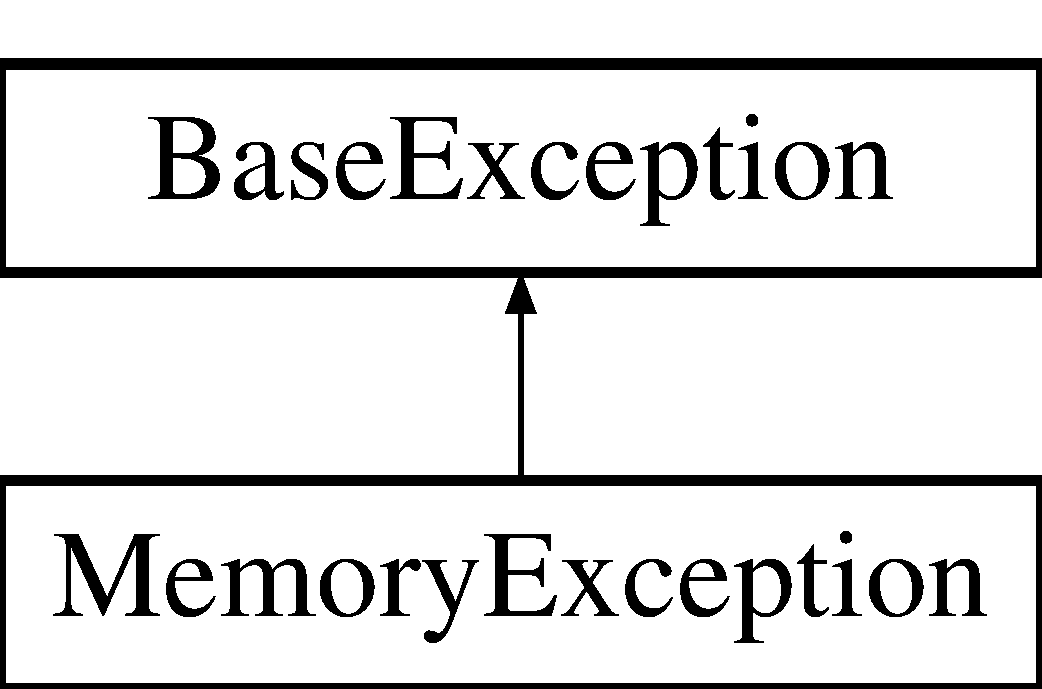
\includegraphics[height=2.000000cm]{structMemoryException}
\end{center}
\end{figure}
\subsection*{Public Member Functions}
\begin{DoxyCompactItemize}
\item 
\hyperlink{structMemoryException_a06ee326a263f05bdc51b1fd77864a0f5}{MemoryException} (const std::string \&val)
\end{DoxyCompactItemize}


\subsection{Detailed Description}
Memory exception if the user requires less than 0 or more than all of the memory. 

Definition at line 40 of file Exceptions.h.



\subsection{Constructor \& Destructor Documentation}
\hypertarget{structMemoryException_a06ee326a263f05bdc51b1fd77864a0f5}{
\index{MemoryException@{MemoryException}!MemoryException@{MemoryException}}
\index{MemoryException@{MemoryException}!MemoryException@{MemoryException}}
\subsubsection[{MemoryException}]{\setlength{\rightskip}{0pt plus 5cm}MemoryException::MemoryException (
\begin{DoxyParamCaption}
\item[{const std::string \&}]{ val}
\end{DoxyParamCaption}
)\hspace{0.3cm}{\ttfamily  \mbox{[}inline\mbox{]}}}}
\label{structMemoryException_a06ee326a263f05bdc51b1fd77864a0f5}


Definition at line 42 of file Exceptions.h.



The documentation for this struct was generated from the following file:\begin{DoxyCompactItemize}
\item 
include/\hyperlink{Exceptions_8h}{Exceptions.h}\end{DoxyCompactItemize}

\hypertarget{structObjectNotFound}{
\section{ObjectNotFound Struct Reference}
\label{structObjectNotFound}\index{ObjectNotFound@{ObjectNotFound}}
}


Thrown if the selected object is not in the file.  




{\ttfamily \#include $<$Exceptions.h$>$}

Inheritance diagram for ObjectNotFound:\begin{figure}[H]
\begin{center}
\leavevmode
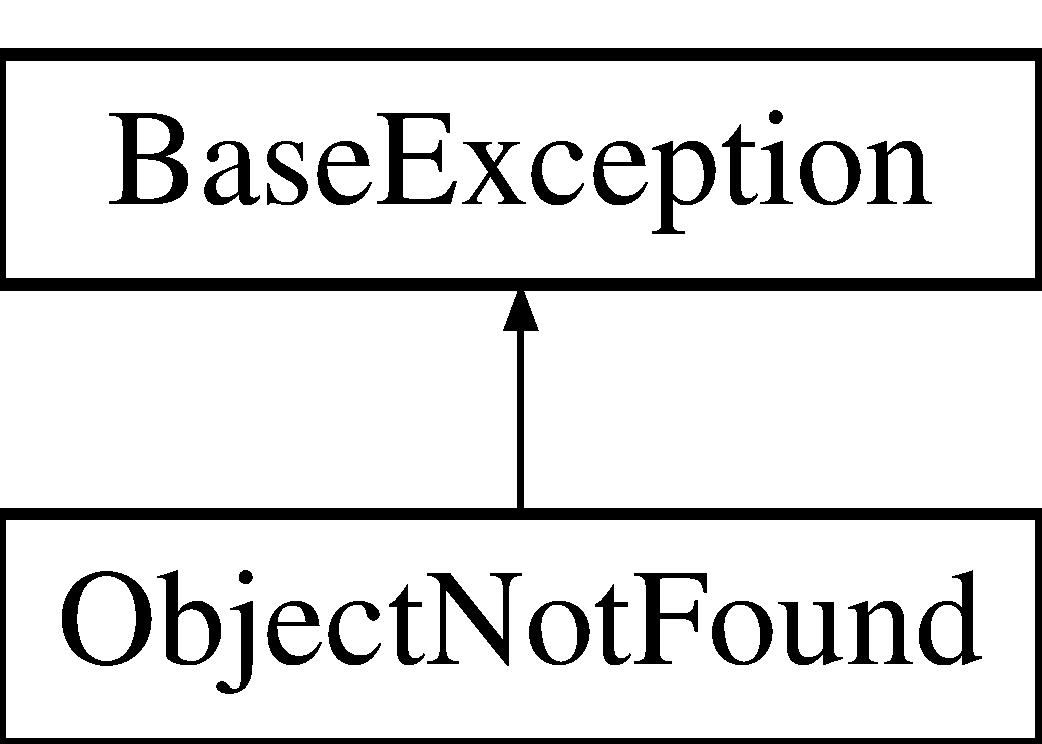
\includegraphics[height=2.000000cm]{structObjectNotFound}
\end{center}
\end{figure}
\subsection*{Public Member Functions}
\begin{DoxyCompactItemize}
\item 
\hyperlink{structObjectNotFound_ac2aa4da353b1fb177298dd41810664ff}{ObjectNotFound} (const std::string \&val)
\end{DoxyCompactItemize}


\subsection{Detailed Description}
Thrown if the selected object is not in the file. 

Definition at line 28 of file Exceptions.h.



\subsection{Constructor \& Destructor Documentation}
\hypertarget{structObjectNotFound_ac2aa4da353b1fb177298dd41810664ff}{
\index{ObjectNotFound@{ObjectNotFound}!ObjectNotFound@{ObjectNotFound}}
\index{ObjectNotFound@{ObjectNotFound}!ObjectNotFound@{ObjectNotFound}}
\subsubsection[{ObjectNotFound}]{\setlength{\rightskip}{0pt plus 5cm}ObjectNotFound::ObjectNotFound (
\begin{DoxyParamCaption}
\item[{const std::string \&}]{ val}
\end{DoxyParamCaption}
)\hspace{0.3cm}{\ttfamily  \mbox{[}inline\mbox{]}}}}
\label{structObjectNotFound_ac2aa4da353b1fb177298dd41810664ff}


Definition at line 30 of file Exceptions.h.



The documentation for this struct was generated from the following file:\begin{DoxyCompactItemize}
\item 
include/\hyperlink{Exceptions_8h}{Exceptions.h}\end{DoxyCompactItemize}

\hypertarget{structXMLException}{
\section{XMLException Struct Reference}
\label{structXMLException}\index{XMLException@{XMLException}}
}


Custom xml exception if any xml handling goes wrong.  




{\ttfamily \#include $<$Exceptions.h$>$}

Inheritance diagram for XMLException:\begin{figure}[H]
\begin{center}
\leavevmode
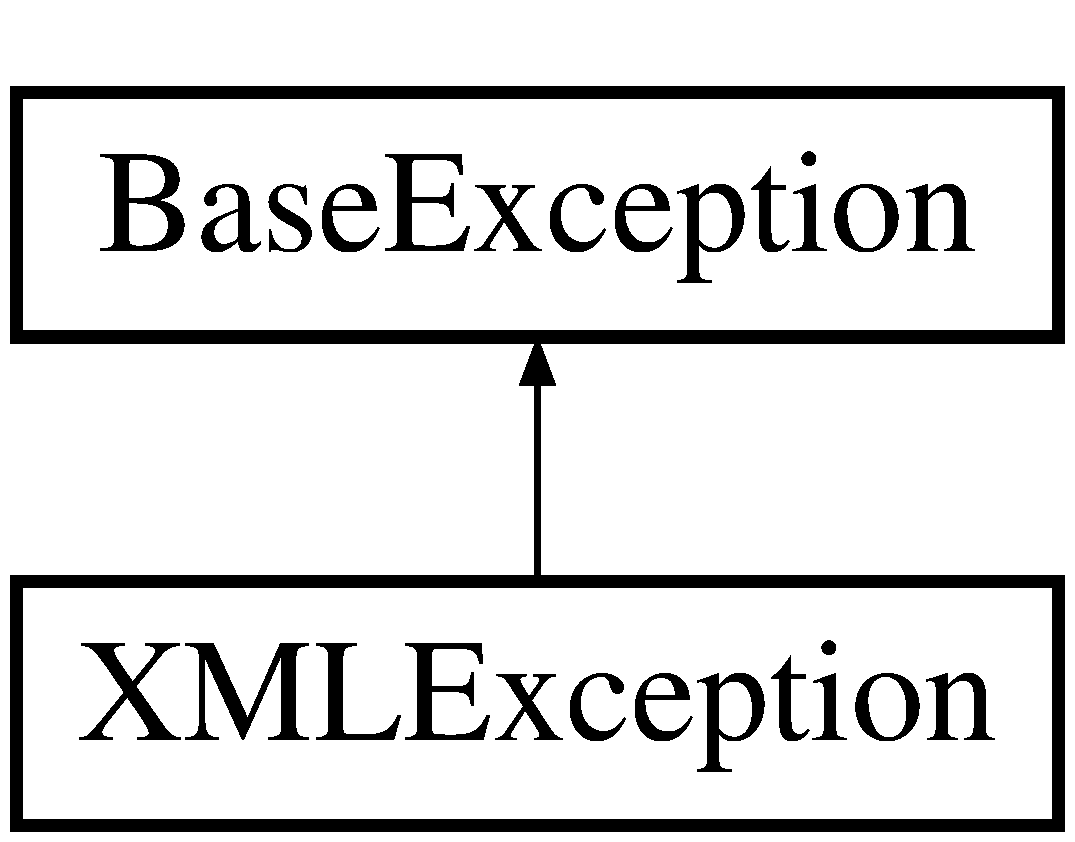
\includegraphics[height=2.000000cm]{structXMLException}
\end{center}
\end{figure}
\subsection*{Public Member Functions}
\begin{DoxyCompactItemize}
\item 
\hyperlink{structXMLException_a64b9a0ee1a27c68d661c70c6e8a8a739}{XMLException} (const std::string \&val)
\end{DoxyCompactItemize}


\subsection{Detailed Description}
Custom xml exception if any xml handling goes wrong. 

Definition at line 34 of file Exceptions.h.



\subsection{Constructor \& Destructor Documentation}
\hypertarget{structXMLException_a64b9a0ee1a27c68d661c70c6e8a8a739}{
\index{XMLException@{XMLException}!XMLException@{XMLException}}
\index{XMLException@{XMLException}!XMLException@{XMLException}}
\subsubsection[{XMLException}]{\setlength{\rightskip}{0pt plus 5cm}XMLException::XMLException (
\begin{DoxyParamCaption}
\item[{const std::string \&}]{ val}
\end{DoxyParamCaption}
)\hspace{0.3cm}{\ttfamily  \mbox{[}inline\mbox{]}}}}
\label{structXMLException_a64b9a0ee1a27c68d661c70c6e8a8a739}


Definition at line 36 of file Exceptions.h.



The documentation for this struct was generated from the following file:\begin{DoxyCompactItemize}
\item 
include/\hyperlink{Exceptions_8h}{Exceptions.h}\end{DoxyCompactItemize}

\chapter{File Documentation}
\hypertarget{AlterTransit_8h}{
\section{include/AlterTransit.h File Reference}
\label{AlterTransit_8h}\index{include/AlterTransit.h@{include/AlterTransit.h}}
}
{\ttfamily \#include \char`\"{}Lightcurve.h\char`\"{}}\par
\subsection*{Functions}
\begin{DoxyCompactItemize}
\item 
\hyperlink{classLightcurve}{Lightcurve} \hyperlink{AlterTransit_8h_a3a8c7372713c9dea27e5a8e81f365acb}{RemoveTransit} (\hyperlink{classLightcurve}{Lightcurve} \&data, \hyperlink{classLightcurve}{Lightcurve} \&model)
\item 
\hyperlink{classLightcurve}{Lightcurve} \hyperlink{AlterTransit_8h_abeb36a203c65247c1c9b69009be575c7}{AddTransit} (\hyperlink{classLightcurve}{Lightcurve} \&data, \hyperlink{classLightcurve}{Lightcurve} \&model)
\item 
\hyperlink{classLightcurve}{Lightcurve} \hyperlink{AlterTransit_8h_a96ad7d61a1ef55f93aa8234d3184148e}{AlterTransit} (\hyperlink{classLightcurve}{Lightcurve} \&data, \hyperlink{classLightcurve}{Lightcurve} \&subModel, \hyperlink{classLightcurve}{Lightcurve} \&addModel, bool WASP, bool addModelFlag=true)
\end{DoxyCompactItemize}


\subsection{Function Documentation}
\hypertarget{AlterTransit_8h_abeb36a203c65247c1c9b69009be575c7}{
\index{AlterTransit.h@{AlterTransit.h}!AddTransit@{AddTransit}}
\index{AddTransit@{AddTransit}!AlterTransit.h@{AlterTransit.h}}
\subsubsection[{AddTransit}]{\setlength{\rightskip}{0pt plus 5cm}{\bf Lightcurve} AddTransit (
\begin{DoxyParamCaption}
\item[{{\bf Lightcurve} \&}]{ data, }
\item[{{\bf Lightcurve} \&}]{ model}
\end{DoxyParamCaption}
)}}
\label{AlterTransit_8h_abeb36a203c65247c1c9b69009be575c7}
\hypertarget{AlterTransit_8h_a96ad7d61a1ef55f93aa8234d3184148e}{
\index{AlterTransit.h@{AlterTransit.h}!AlterTransit@{AlterTransit}}
\index{AlterTransit@{AlterTransit}!AlterTransit.h@{AlterTransit.h}}
\subsubsection[{AlterTransit}]{\setlength{\rightskip}{0pt plus 5cm}{\bf Lightcurve} AlterTransit (
\begin{DoxyParamCaption}
\item[{{\bf Lightcurve} \&}]{ data, }
\item[{{\bf Lightcurve} \&}]{ subModel, }
\item[{{\bf Lightcurve} \&}]{ addModel, }
\item[{bool}]{ WASP, }
\item[{bool}]{ addModelFlag = {\ttfamily true}}
\end{DoxyParamCaption}
)}}
\label{AlterTransit_8h_a96ad7d61a1ef55f93aa8234d3184148e}
\hypertarget{AlterTransit_8h_a3a8c7372713c9dea27e5a8e81f365acb}{
\index{AlterTransit.h@{AlterTransit.h}!RemoveTransit@{RemoveTransit}}
\index{RemoveTransit@{RemoveTransit}!AlterTransit.h@{AlterTransit.h}}
\subsubsection[{RemoveTransit}]{\setlength{\rightskip}{0pt plus 5cm}{\bf Lightcurve} RemoveTransit (
\begin{DoxyParamCaption}
\item[{{\bf Lightcurve} \&}]{ data, }
\item[{{\bf Lightcurve} \&}]{ model}
\end{DoxyParamCaption}
)}}
\label{AlterTransit_8h_a3a8c7372713c9dea27e5a8e81f365acb}

\hypertarget{Application_8h}{
\section{include/Application.h File Reference}
\label{Application_8h}\index{include/Application.h@{include/Application.h}}
}
{\ttfamily \#include $<$CCfits/CCfits$>$}\par
{\ttfamily \#include \char`\"{}Lightcurve.h\char`\"{}}\par
\subsection*{Classes}
\begin{DoxyCompactItemize}
\item 
class \hyperlink{classApplication}{Application}
\begin{DoxyCompactList}\small\item\em Main class for the program. \item\end{DoxyCompactList}\end{DoxyCompactItemize}

\hypertarget{constants_8h}{
\section{include/constants.h File Reference}
\label{constants_8h}\index{include/constants.h@{include/constants.h}}
}
\subsection*{Variables}
\begin{DoxyCompactItemize}
\item 
const double \hyperlink{constants_8h_a1e6717330dba5c6c109244342f2061b6}{rJup} = 71492E3
\item 
const double \hyperlink{constants_8h_a09e30b17f2999f9024f3912bd42732cc}{rSun} = 6.995E8
\item 
const double \hyperlink{constants_8h_a2b9e1ccc1a034cb26b9c794767315346}{AU} = 1.496E11
\item 
const double \hyperlink{constants_8h_af2ca59800ec0d6ccaaa074e736a455f0}{secondsInMinute} = 60.
\item 
const double \hyperlink{constants_8h_a45af869d90ad2d0a9debdd510e2bd706}{secondsInHour} = 60. $\ast$ \hyperlink{constants_8h_af2ca59800ec0d6ccaaa074e736a455f0}{secondsInMinute}
\item 
const double \hyperlink{constants_8h_a6b663049f298a15759c0d0272f096975}{secondsInDay} = 24. $\ast$ \hyperlink{constants_8h_a45af869d90ad2d0a9debdd510e2bd706}{secondsInHour}
\item 
const double \hyperlink{constants_8h_a41e5a0b51961a3b7cc72a7e4a98dd2b5}{radiansInDegree} = 2. $\ast$ 3.14 / 360.
\item 
const double \hyperlink{constants_8h_a83bf802e458b1e113bc14a9ceb1b2800}{degreesInRadian} = 360. / 2. / 3.14
\end{DoxyCompactItemize}


\subsection{Variable Documentation}
\hypertarget{constants_8h_a2b9e1ccc1a034cb26b9c794767315346}{
\index{constants.h@{constants.h}!AU@{AU}}
\index{AU@{AU}!constants.h@{constants.h}}
\subsubsection[{AU}]{\setlength{\rightskip}{0pt plus 5cm}const double {\bf AU} = 1.496E11}}
\label{constants_8h_a2b9e1ccc1a034cb26b9c794767315346}


Definition at line 6 of file constants.h.

\hypertarget{constants_8h_a83bf802e458b1e113bc14a9ceb1b2800}{
\index{constants.h@{constants.h}!degreesInRadian@{degreesInRadian}}
\index{degreesInRadian@{degreesInRadian}!constants.h@{constants.h}}
\subsubsection[{degreesInRadian}]{\setlength{\rightskip}{0pt plus 5cm}const double {\bf degreesInRadian} = 360. / 2. / 3.14}}
\label{constants_8h_a83bf802e458b1e113bc14a9ceb1b2800}


Definition at line 11 of file constants.h.

\hypertarget{constants_8h_a41e5a0b51961a3b7cc72a7e4a98dd2b5}{
\index{constants.h@{constants.h}!radiansInDegree@{radiansInDegree}}
\index{radiansInDegree@{radiansInDegree}!constants.h@{constants.h}}
\subsubsection[{radiansInDegree}]{\setlength{\rightskip}{0pt plus 5cm}const double {\bf radiansInDegree} = 2. $\ast$ 3.14 / 360.}}
\label{constants_8h_a41e5a0b51961a3b7cc72a7e4a98dd2b5}


Definition at line 10 of file constants.h.

\hypertarget{constants_8h_a1e6717330dba5c6c109244342f2061b6}{
\index{constants.h@{constants.h}!rJup@{rJup}}
\index{rJup@{rJup}!constants.h@{constants.h}}
\subsubsection[{rJup}]{\setlength{\rightskip}{0pt plus 5cm}const double {\bf rJup} = 71492E3}}
\label{constants_8h_a1e6717330dba5c6c109244342f2061b6}


Definition at line 4 of file constants.h.

\hypertarget{constants_8h_a09e30b17f2999f9024f3912bd42732cc}{
\index{constants.h@{constants.h}!rSun@{rSun}}
\index{rSun@{rSun}!constants.h@{constants.h}}
\subsubsection[{rSun}]{\setlength{\rightskip}{0pt plus 5cm}const double {\bf rSun} = 6.995E8}}
\label{constants_8h_a09e30b17f2999f9024f3912bd42732cc}


Definition at line 5 of file constants.h.

\hypertarget{constants_8h_a6b663049f298a15759c0d0272f096975}{
\index{constants.h@{constants.h}!secondsInDay@{secondsInDay}}
\index{secondsInDay@{secondsInDay}!constants.h@{constants.h}}
\subsubsection[{secondsInDay}]{\setlength{\rightskip}{0pt plus 5cm}const double {\bf secondsInDay} = 24. $\ast$ {\bf secondsInHour}}}
\label{constants_8h_a6b663049f298a15759c0d0272f096975}


Definition at line 9 of file constants.h.

\hypertarget{constants_8h_a45af869d90ad2d0a9debdd510e2bd706}{
\index{constants.h@{constants.h}!secondsInHour@{secondsInHour}}
\index{secondsInHour@{secondsInHour}!constants.h@{constants.h}}
\subsubsection[{secondsInHour}]{\setlength{\rightskip}{0pt plus 5cm}const double {\bf secondsInHour} = 60. $\ast$ {\bf secondsInMinute}}}
\label{constants_8h_a45af869d90ad2d0a9debdd510e2bd706}


Definition at line 8 of file constants.h.

\hypertarget{constants_8h_af2ca59800ec0d6ccaaa074e736a455f0}{
\index{constants.h@{constants.h}!secondsInMinute@{secondsInMinute}}
\index{secondsInMinute@{secondsInMinute}!constants.h@{constants.h}}
\subsubsection[{secondsInMinute}]{\setlength{\rightskip}{0pt plus 5cm}const double {\bf secondsInMinute} = 60.}}
\label{constants_8h_af2ca59800ec0d6ccaaa074e736a455f0}


Definition at line 7 of file constants.h.


\hypertarget{Exceptions_8h}{
\section{include/Exceptions.h File Reference}
\label{Exceptions_8h}\index{include/Exceptions.h@{include/Exceptions.h}}
}
{\ttfamily \#include $<$exception$>$}\par
{\ttfamily \#include $<$string$>$}\par
\subsection*{Classes}
\begin{DoxyCompactItemize}
\item 
struct \hyperlink{structBaseException}{BaseException}
\begin{DoxyCompactList}\small\item\em Base exception. \item\end{DoxyCompactList}\item 
struct \hyperlink{structObjectNotFound}{ObjectNotFound}
\begin{DoxyCompactList}\small\item\em Thrown if the selected object is not in the file. \item\end{DoxyCompactList}\item 
struct \hyperlink{structXMLException}{XMLException}
\begin{DoxyCompactList}\small\item\em Custom xml exception if any xml handling goes wrong. \item\end{DoxyCompactList}\item 
struct \hyperlink{structMemoryException}{MemoryException}
\begin{DoxyCompactList}\small\item\em Memory exception if the user requires less than 0 or more than all of the memory. \item\end{DoxyCompactList}\end{DoxyCompactItemize}

\hypertarget{FuncIntensity_8h}{
\section{include/FuncIntensity.h File Reference}
\label{FuncIntensity_8h}\index{include/FuncIntensity.h@{include/FuncIntensity.h}}
}
{\ttfamily \#include $<$vector$>$}\par
\subsection*{Functions}
\begin{DoxyCompactItemize}
\item 
double \hyperlink{FuncIntensity_8h_a7218240bfa5bdbb25b53f2b6cbce8e17}{I} (double r, double c1, double c2, double c3, double c4)
\item 
double \hyperlink{FuncIntensity_8h_a9e68683166841e0d508360994e8f9947}{I} (double r, const std::vector$<$ double $>$ \&coeffs)
\item 
double \hyperlink{FuncIntensity_8h_a80ec5ddc0c4a5ad934b5e207727ccf69}{IntegratedI} (double dr, double c1, double c2, double c3, double c4, double rlow, double rhigh)
\item 
double \hyperlink{FuncIntensity_8h_ab2c7e855fa46644b8ef739901d8d330b}{IntegratedI} (double dr, const std::vector$<$ double $>$ \&coeffs, double rlow, double rhigh)
\end{DoxyCompactItemize}


\subsection{Function Documentation}
\hypertarget{FuncIntensity_8h_a7218240bfa5bdbb25b53f2b6cbce8e17}{
\index{FuncIntensity.h@{FuncIntensity.h}!I@{I}}
\index{I@{I}!FuncIntensity.h@{FuncIntensity.h}}
\subsubsection[{I}]{\setlength{\rightskip}{0pt plus 5cm}double I (
\begin{DoxyParamCaption}
\item[{double}]{ r, }
\item[{double}]{ c1, }
\item[{double}]{ c2, }
\item[{double}]{ c3, }
\item[{double}]{ c4}
\end{DoxyParamCaption}
)}}
\label{FuncIntensity_8h_a7218240bfa5bdbb25b53f2b6cbce8e17}
\hypertarget{FuncIntensity_8h_a9e68683166841e0d508360994e8f9947}{
\index{FuncIntensity.h@{FuncIntensity.h}!I@{I}}
\index{I@{I}!FuncIntensity.h@{FuncIntensity.h}}
\subsubsection[{I}]{\setlength{\rightskip}{0pt plus 5cm}double I (
\begin{DoxyParamCaption}
\item[{double}]{ r, }
\item[{const std::vector$<$ double $>$ \&}]{ coeffs}
\end{DoxyParamCaption}
)}}
\label{FuncIntensity_8h_a9e68683166841e0d508360994e8f9947}
\hypertarget{FuncIntensity_8h_a80ec5ddc0c4a5ad934b5e207727ccf69}{
\index{FuncIntensity.h@{FuncIntensity.h}!IntegratedI@{IntegratedI}}
\index{IntegratedI@{IntegratedI}!FuncIntensity.h@{FuncIntensity.h}}
\subsubsection[{IntegratedI}]{\setlength{\rightskip}{0pt plus 5cm}double IntegratedI (
\begin{DoxyParamCaption}
\item[{double}]{ dr, }
\item[{double}]{ c1, }
\item[{double}]{ c2, }
\item[{double}]{ c3, }
\item[{double}]{ c4, }
\item[{double}]{ rlow, }
\item[{double}]{ rhigh}
\end{DoxyParamCaption}
)}}
\label{FuncIntensity_8h_a80ec5ddc0c4a5ad934b5e207727ccf69}
\hypertarget{FuncIntensity_8h_ab2c7e855fa46644b8ef739901d8d330b}{
\index{FuncIntensity.h@{FuncIntensity.h}!IntegratedI@{IntegratedI}}
\index{IntegratedI@{IntegratedI}!FuncIntensity.h@{FuncIntensity.h}}
\subsubsection[{IntegratedI}]{\setlength{\rightskip}{0pt plus 5cm}double IntegratedI (
\begin{DoxyParamCaption}
\item[{double}]{ dr, }
\item[{const std::vector$<$ double $>$ \&}]{ coeffs, }
\item[{double}]{ rlow, }
\item[{double}]{ rhigh}
\end{DoxyParamCaption}
)}}
\label{FuncIntensity_8h_ab2c7e855fa46644b8ef739901d8d330b}

\hypertarget{FuncOmega_8h}{
\section{include/FuncOmega.h File Reference}
\label{FuncOmega_8h}\index{include/FuncOmega.h@{include/FuncOmega.h}}
}
{\ttfamily \#include $<$vector$>$}\par
\subsection*{Functions}
\begin{DoxyCompactItemize}
\item 
double \hyperlink{FuncOmega_8h_a1b4949a804ec7f75f05bc8e8c8ac5b7a}{calcOmega} (const std::vector$<$ double $>$ \&coeffs)
\end{DoxyCompactItemize}


\subsection{Function Documentation}
\hypertarget{FuncOmega_8h_a1b4949a804ec7f75f05bc8e8c8ac5b7a}{
\index{FuncOmega.h@{FuncOmega.h}!calcOmega@{calcOmega}}
\index{calcOmega@{calcOmega}!FuncOmega.h@{FuncOmega.h}}
\subsubsection[{calcOmega}]{\setlength{\rightskip}{0pt plus 5cm}double calcOmega (
\begin{DoxyParamCaption}
\item[{const std::vector$<$ double $>$ \&}]{ coeffs}
\end{DoxyParamCaption}
)}}
\label{FuncOmega_8h_a1b4949a804ec7f75f05bc8e8c8ac5b7a}

\hypertarget{FuncSquare_8h}{
\section{include/FuncSquare.h File Reference}
\label{FuncSquare_8h}\index{include/FuncSquare.h@{include/FuncSquare.h}}
}
\subsection*{Functions}
\begin{DoxyCompactItemize}
\item 
{\footnotesize template$<$class T $>$ }\\T \hyperlink{FuncSquare_8h_a9396ef05d06a94353526b1b34e6c36fc}{square} (T val)
\end{DoxyCompactItemize}


\subsection{Function Documentation}
\hypertarget{FuncSquare_8h_a9396ef05d06a94353526b1b34e6c36fc}{
\index{FuncSquare.h@{FuncSquare.h}!square@{square}}
\index{square@{square}!FuncSquare.h@{FuncSquare.h}}
\subsubsection[{square}]{\setlength{\rightskip}{0pt plus 5cm}template$<$class T $>$ T square (
\begin{DoxyParamCaption}
\item[{T}]{ val}
\end{DoxyParamCaption}
)\hspace{0.3cm}{\ttfamily  \mbox{[}inline\mbox{]}}}}
\label{FuncSquare_8h_a9396ef05d06a94353526b1b34e6c36fc}


Definition at line 4 of file FuncSquare.h.


\hypertarget{GetSystemMemory_8h}{
\section{include/GetSystemMemory.h File Reference}
\label{GetSystemMemory_8h}\index{include/GetSystemMemory.h@{include/GetSystemMemory.h}}
}
\subsection*{Functions}
\begin{DoxyCompactItemize}
\item 
long \hyperlink{GetSystemMemory_8h_a61801d4d0fd0a0b0de1dfed288dbb120}{getTotalSystemMemory} ()
\begin{DoxyCompactList}\small\item\em Returns the system memory. \item\end{DoxyCompactList}\end{DoxyCompactItemize}


\subsection{Function Documentation}
\hypertarget{GetSystemMemory_8h_a61801d4d0fd0a0b0de1dfed288dbb120}{
\index{GetSystemMemory.h@{GetSystemMemory.h}!getTotalSystemMemory@{getTotalSystemMemory}}
\index{getTotalSystemMemory@{getTotalSystemMemory}!GetSystemMemory.h@{GetSystemMemory.h}}
\subsubsection[{getTotalSystemMemory}]{\setlength{\rightskip}{0pt plus 5cm}long getTotalSystemMemory (
\begin{DoxyParamCaption}
{}
\end{DoxyParamCaption}
)}}
\label{GetSystemMemory_8h_a61801d4d0fd0a0b0de1dfed288dbb120}


Returns the system memory. 

Runs platform independant (on apple and linux anyway) method of getting the system memory (RAM) in bytes 
\hypertarget{Lightcurve_8h}{
\section{include/Lightcurve.h File Reference}
\label{Lightcurve_8h}\index{include/Lightcurve.h@{include/Lightcurve.h}}
}
{\ttfamily \#include $<$vector$>$}\par
\subsection*{Classes}
\begin{DoxyCompactItemize}
\item 
class \hyperlink{classLightcurve}{Lightcurve}
\begin{DoxyCompactList}\small\item\em \hyperlink{classLightcurve}{Lightcurve} class which stores information about a single object. \item\end{DoxyCompactList}\end{DoxyCompactItemize}

\hypertarget{SortedIndex_8h}{
\section{include/SortedIndex.h File Reference}
\label{SortedIndex_8h}\index{include/SortedIndex.h@{include/SortedIndex.h}}
}
{\ttfamily \#include $<$algorithm$>$}\par
{\ttfamily \#include $<$nr/nr3.h$>$}\par
{\ttfamily \#include $<$nr/interp\_\-1d.h$>$}\par
{\ttfamily \#include $<$nr/interp\_\-linear.h$>$}\par
\subsection*{Defines}
\begin{DoxyCompactItemize}
\item 
\#define \hyperlink{SortedIndex_8h_aa70f69e9467dbd77cd635ce6f7fb55a8}{\_\-USESTDVECTOR\_\-}
\end{DoxyCompactItemize}
\subsection*{Functions}
\begin{DoxyCompactItemize}
\item 
bool \hyperlink{SortedIndex_8h_af49fc875aefc8df73eb55ae68a28c03e}{PairComparitor} (const pair$<$ double, int $>$ \&val1, const pair$<$ double, int $>$ \&val2)
\item 
{\footnotesize template$<$typename T $>$ }\\std::vector$<$ std::pair$<$ double, int $>$ $>$ \hyperlink{SortedIndex_8h_a736118672339a2b9ed2ab3caef757a7c}{SortedIndex} (const std::vector$<$ T $>$ \&data)
\end{DoxyCompactItemize}


\subsection{Define Documentation}
\hypertarget{SortedIndex_8h_aa70f69e9467dbd77cd635ce6f7fb55a8}{
\index{SortedIndex.h@{SortedIndex.h}!\_\-USESTDVECTOR\_\-@{\_\-USESTDVECTOR\_\-}}
\index{\_\-USESTDVECTOR\_\-@{\_\-USESTDVECTOR\_\-}!SortedIndex.h@{SortedIndex.h}}
\subsubsection[{\_\-USESTDVECTOR\_\-}]{\setlength{\rightskip}{0pt plus 5cm}\#define \_\-USESTDVECTOR\_\-}}
\label{SortedIndex_8h_aa70f69e9467dbd77cd635ce6f7fb55a8}


Definition at line 9 of file SortedIndex.h.



\subsection{Function Documentation}
\hypertarget{SortedIndex_8h_af49fc875aefc8df73eb55ae68a28c03e}{
\index{SortedIndex.h@{SortedIndex.h}!PairComparitor@{PairComparitor}}
\index{PairComparitor@{PairComparitor}!SortedIndex.h@{SortedIndex.h}}
\subsubsection[{PairComparitor}]{\setlength{\rightskip}{0pt plus 5cm}bool PairComparitor (
\begin{DoxyParamCaption}
\item[{const pair$<$ double, int $>$ \&}]{ val1, }
\item[{const pair$<$ double, int $>$ \&}]{ val2}
\end{DoxyParamCaption}
)}}
\label{SortedIndex_8h_af49fc875aefc8df73eb55ae68a28c03e}


Definition at line 16 of file SortedIndex.h.

\hypertarget{SortedIndex_8h_a736118672339a2b9ed2ab3caef757a7c}{
\index{SortedIndex.h@{SortedIndex.h}!SortedIndex@{SortedIndex}}
\index{SortedIndex@{SortedIndex}!SortedIndex.h@{SortedIndex.h}}
\subsubsection[{SortedIndex}]{\setlength{\rightskip}{0pt plus 5cm}template$<$typename T $>$ std::vector$<$std::pair$<$double, int$>$ $>$ SortedIndex (
\begin{DoxyParamCaption}
\item[{const std::vector$<$ T $>$ \&}]{ data}
\end{DoxyParamCaption}
)}}
\label{SortedIndex_8h_a736118672339a2b9ed2ab3caef757a7c}


Definition at line 22 of file SortedIndex.h.


\hypertarget{ToStringList_8h}{
\section{include/ToStringList.h File Reference}
\label{ToStringList_8h}\index{include/ToStringList.h@{include/ToStringList.h}}
}
{\ttfamily \#include $<$vector$>$}\par
{\ttfamily \#include $<$string$>$}\par
{\ttfamily \#include $<$sstream$>$}\par
{\ttfamily \#include $<$CCfits/CCfits$>$}\par
\subsection*{Functions}
\begin{DoxyCompactItemize}
\item 
{\footnotesize template$<$typename T $>$ }\\std::vector$<$ std::string $>$ \hyperlink{ToStringList_8h_af325ea02e2c45bd98a3d0cfab00138bc}{ToStringList} (CCfits::Column \&col, int size)
\end{DoxyCompactItemize}


\subsection{Function Documentation}
\hypertarget{ToStringList_8h_af325ea02e2c45bd98a3d0cfab00138bc}{
\index{ToStringList.h@{ToStringList.h}!ToStringList@{ToStringList}}
\index{ToStringList@{ToStringList}!ToStringList.h@{ToStringList.h}}
\subsubsection[{ToStringList}]{\setlength{\rightskip}{0pt plus 5cm}template$<$typename T $>$ std::vector$<$std::string$>$ ToStringList (
\begin{DoxyParamCaption}
\item[{CCfits::Column \&}]{ col, }
\item[{int}]{ size}
\end{DoxyParamCaption}
)}}
\label{ToStringList_8h_af325ea02e2c45bd98a3d0cfab00138bc}


Definition at line 12 of file ToStringList.h.


\hypertarget{WaspDateConverter_8h}{
\section{include/WaspDateConverter.h File Reference}
\label{WaspDateConverter_8h}\index{include/WaspDateConverter.h@{include/WaspDateConverter.h}}
}
{\ttfamily \#include \char`\"{}constants.h\char`\"{}}\par
\subsection*{Functions}
\begin{DoxyCompactItemize}
\item 
{\footnotesize template$<$typename T $>$ }\\double \hyperlink{WaspDateConverter_8h_ae66cfa0c23e041a77dcfed6a7940cc87}{wd2jd} (T wd)
\item 
{\footnotesize template$<$typename T $>$ }\\double \hyperlink{WaspDateConverter_8h_aa43c8eca2ad808f69a88ea5c6e8f1e17}{jd2wd} (T jd)
\end{DoxyCompactItemize}


\subsection{Function Documentation}
\hypertarget{WaspDateConverter_8h_aa43c8eca2ad808f69a88ea5c6e8f1e17}{
\index{WaspDateConverter.h@{WaspDateConverter.h}!jd2wd@{jd2wd}}
\index{jd2wd@{jd2wd}!WaspDateConverter.h@{WaspDateConverter.h}}
\subsubsection[{jd2wd}]{\setlength{\rightskip}{0pt plus 5cm}template$<$typename T $>$ double jd2wd (
\begin{DoxyParamCaption}
\item[{T}]{ jd}
\end{DoxyParamCaption}
)\hspace{0.3cm}{\ttfamily  \mbox{[}inline\mbox{]}}}}
\label{WaspDateConverter_8h_aa43c8eca2ad808f69a88ea5c6e8f1e17}


Definition at line 16 of file WaspDateConverter.h.

\hypertarget{WaspDateConverter_8h_ae66cfa0c23e041a77dcfed6a7940cc87}{
\index{WaspDateConverter.h@{WaspDateConverter.h}!wd2jd@{wd2jd}}
\index{wd2jd@{wd2jd}!WaspDateConverter.h@{WaspDateConverter.h}}
\subsubsection[{wd2jd}]{\setlength{\rightskip}{0pt plus 5cm}template$<$typename T $>$ double wd2jd (
\begin{DoxyParamCaption}
\item[{T}]{ wd}
\end{DoxyParamCaption}
)\hspace{0.3cm}{\ttfamily  \mbox{[}inline\mbox{]}}}}
\label{WaspDateConverter_8h_ae66cfa0c23e041a77dcfed6a7940cc87}


Definition at line 8 of file WaspDateConverter.h.


\hypertarget{XMLParserPugi_8h}{
\section{include/XMLParserPugi.h File Reference}
\label{XMLParserPugi_8h}\index{include/XMLParserPugi.h@{include/XMLParserPugi.h}}
}
{\ttfamily \#include $<$pugixml.hpp$>$}\par
{\ttfamily \#include $<$vector$>$}\par
{\ttfamily \#include $<$string$>$}\par
\subsection*{Classes}
\begin{DoxyCompactItemize}
\item 
class \hyperlink{classConfig_1_1Config}{Config::Config}
\begin{DoxyCompactList}\small\item\em XML configuration file parser. \item\end{DoxyCompactList}\end{DoxyCompactItemize}
\subsection*{Namespaces}
\begin{DoxyCompactItemize}
\item 
namespace \hyperlink{namespaceConfig}{Config}


\begin{DoxyCompactList}\small\item\em \hyperlink{namespaceConfig}{Config} namespace to keep the configuration parser seperate. \item\end{DoxyCompactList}

\end{DoxyCompactItemize}

\printindex
\end{document}
